\documentclass[10pt, a4paper, spanish]{article}
\usepackage[paper=a4paper, left=1.5cm, right=1.5cm, bottom=1.5cm, top=3.5cm]{geometry}
\usepackage[utf8]{inputenc}
\usepackage[spanish]{babel}
\usepackage[]{caratula}
\usepackage[pdfencoding=auto, colorlinks=true, linkcolor=blue]{hyperref}
\usepackage[table,xcdraw]{xcolor}
\usepackage{tikz}
\usetikzlibrary{matrix}
\usepackage{graphicx}
\usepackage{subcaption}
\usepackage{amsmath}
\usepackage{float}
\usepackage{listings}

\definecolor{commentgreen}{RGB}{2,112,10}
\definecolor{eminence}{RGB}{108,48,130}
\definecolor{weborange}{RGB}{255,165,0}
\definecolor{frenchplum}{RGB}{129,20,83}
\lstset {
    language=C,
    frame=tb,
    tabsize=4,
    showstringspaces=false,
    numbers=left,
    %upquote=true,
    commentstyle=\color{commentgreen},
    keywordstyle=\color{eminence},
    stringstyle=\color{red},
    basicstyle=\small\ttfamily, % basic font setting
    emph={int,char,double,float,unsigned,void,bool},
    emphstyle={\color{blue}},
    escapechar=\&,
    % keyword highlighting
    classoffset=1, % starting new class
    otherkeywords={>,<,.,;,-,!,=,~},
    morekeywords={>,<,.,;,-,!,=,~},
    keywordstyle=\color{weborange},
    classoffset=0,
}

\newcommand\complejidad{\textbf{Complejidad}}
\newcommand\justifcomp{\textbf{Justificación}}
\newcommand\OdeLinea[1]{\Comment*[r]{$O(#1)$}}
\newcommand\OdeBloque[1]{\Comment*[f]{$O(#1)$}}

\newcommand{\TituloDis}[1]{
  \vspace*{1ex}\par\noindent\textbf{\large #1}\par
}

\newcommand{\algoritmo}[3]{\hangindent=\parindent#1 (#2) \ifx#3\empty\else$\rightarrow$ res: #3\fi}


\newcommand{\mm}[1]{\texttt{MM$_{#1}$}\ }
\newcommand{\xmm}[1]{\texttt{XMM$_{#1}$}\ }
\newcommand{\ymm}[1]{\texttt{YMM$_{#1}$}\ }
\newcommand{\rax}{\texttt{RAX}\ }
\newcommand{\rbx}{\texttt{RBX}\ }
\newcommand{\rcx}{\texttt{RCX}\ }
\newcommand{\rdx}{\texttt{RDX}\ }
\newcommand{\rbp}{\texttt{RBP}\ }
\newcommand{\rsp}{\texttt{RSP}\ }
\newcommand{\reg}[1]{\texttt{R#1}\ }
\newcommand{\asm}[1]{\texttt{\uppercase{#1}}\ }

% ----- Comandos para escribir registros XMM -------------------------------

\usepackage{array}
\newcolumntype{L}[1]{>{\raggedright\let\newline\\\arraybackslash\hspace{0pt}}m{#1}}
\newcolumntype{C}[1]{>{\centering\let\newline\\\arraybackslash\hspace{0pt}}m{#1}}
\newcolumntype{R}[1]{>{\raggedleft\let\newline\\\arraybackslash\hspace{0pt}}m{#1}}

\newcommand{\xmmByte}[8]{
    \def\tempa{#1}
    \def\tempb{#2}
    \def\tempc{#3}
    \def\tempd{#4}
    \def\tempe{#5}
    \def\tempf{#6}
    \def\tempg{#7}
    \def\temph{#8}
    \xmmByteAux
}
\newcommand{\xmmByteAux}[8]{
    \vspace{0.1cm}
    \kern-2em
    \begin{tabular}{|C{0.5cm}|C{0.5cm}|C{0.5cm}|C{0.5cm}|C{0.5cm}|C{0.5cm}|C{0.5cm}|C{0.5cm}|
                     C{0.5cm}|C{0.5cm}|C{0.5cm}|C{0.5cm}|C{0.5cm}|C{0.5cm}|C{0.5cm}|C{0.5cm}|}\hline
    \tempa & \tempb & \tempc & \tempd & \tempe & \tempf & \tempg & \temph &
    #1 & #2 & #3 & #4 & #5 & #6 & #7 & #8 \\ \hline
    \end{tabular}
    \vspace{0.1cm}
}

\newcommand{\xmmWord}[8]{
    \vspace{0.1cm}
    \begin{tabular}{|C{1cm}|C{1cm}|C{1cm}|C{1cm}|C{1cm}|C{1cm}|C{1cm}|C{1cm}|}\hline
    #1 & #2 & #3 & #4 & #5 & #6 & #7 & #8 \\ \hline
    \end{tabular}
    \vspace{0.1cm}
}


\newcommand{\xmmDoubleWord}[4]{
    \vspace{0.1cm}
    \begin{tabular}{|C{3.2cm}|C{3.2cm}|C{3.2cm}|C{3.2cm}|}\hline
    #1 & #2 & #3 & #4 \\ \hline
    \end{tabular}
    \vspace{0.1cm}
}

\newcommand{\xmmDoubleWordSmall}[4]{
    \vspace{0.1cm}
    \begin{tabular}{|C{2cm}|C{2cm}|C{2cm}|C{2cm}|}\hline
    #1 & #2 & #3 & #4 \\ \hline
    \end{tabular}
    \vspace{0.1cm}
}

\newcommand{\xmmQuadWord}[2]{
    \vspace{0.1cm}
    \begin{tabular}{|C{4cm}|C{4cm}|}\hline
    #1 & #2 \\ \hline
    \end{tabular}
    \vspace{0.1cm}
}

\let\xmmFloat\xmmDoubleWord
\let\xmmDouble\xmmQuadWord


\begin{document}


% CARATULA
\materia{Organización del Computador II}
\submateria{Primer Cuatrimestre de 2017}
\fecha{\today}
\titulo{Trabajo Práctico 2}

\integrante{Bonggio, Enzo}{074/15}{ebonggio@dc.uba.ar}
\integrante{?, ?}{?}{?}
\integrante{Tarrío, Ignacio}{363/15}{itarrio@dc.uba.ar}

\maketitle

\tableofcontents
\pagebreak

\section{Convertir entre RGB e YUV}

Los primeros filtros se tratan de conversores entre los espacios de colores RGB e YUV. Los mismos toman los valores de cada pixel y aplican transformaciones matriciales, tomando cada pixel individual como una matriz de sus componentes.

Esta transformación normalmente implica decimales, pero la misma está simplificada para funcionar con enteros entre 0 y 255 (que son los valores posibles de cada componente de un pixel).

Para la conversión RGB a YUV se aplican la siguiente transformación:

\begin{center}

	$
	\begin{bmatrix*}[l]
	Y = sature(((66 * R + 129 * G + 25 * B + 128) >> 8) + 16) \\
	U = sature(((-38 * R - 74 * G + 112 * B + 128) >> 8) + 128) \\
	V = sature(((112 * R - 94 * G - 18 * B + 128) >> 8) + 128)
	\end{bmatrix*}
	$

\end{center}

donde $sature$ representa una saturación sin signo, es decir, los valores fuera del rango [0,255] son acotados a los extremos del mismo.

Para la transformación inversa se utiliza la siguiente transformación:

\begin{center}

	$
	\begin{bmatrix*}[l]
	R = sature((298 * (Y - 16) + 409 * (V - 128) + 128) >> 8) \\
	G = sature((298 * (Y - 16) - 100 * (U - 128) - 208 * (V - 128) + 128) >> 8) \\
	B = sature((298 * (Y - 16) + 516 * (U - 128) + 128) >> 8)
	\end{bmatrix*}
	$

\end{center}

Cabe destacar que si bien los valores son correctos, los visores de imágenes siguen renderizando los colores como si correspondiesen a RGB, por lo que se genera el efecto visual que se muestra a continuación:


\begin{figure}[H]
	\centering
	$\vcenter{\hbox{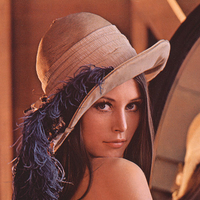
\includegraphics[scale=1]{img/convert_RGB.jpg}}}$
	$\vcenter{\hbox{\LARGE$\xrightleftharpoons[\text{YUVtoRGB}]{\text{RGBtoYUV}}$}}$
	$\vcenter{\hbox{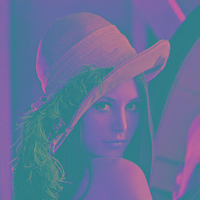
\includegraphics[scale=1]{img/convert_YUV.jpg}}}$
\end{figure}


\subsection{Implementación}

La solución implica recorrer la imagen completa aplicando la transformación a cada pixel de manera individual.

La implementación en C es relativamente trivial: se aplica la transformación correspondiente a cada componente de manera individual. En el caso de la transformación YUV a RGB existen algunos valores que podemos reutilizar, pero los demás cálculos se realizan como se indica en el problema.

Para la implementación en ASM definimos un par de constantes. La idea es que cada una represente una fila de la matriz de transformación. De esta manera, podemos calcular los 3 componentes fuente de cada componente destino en simultaneo.

Para los siguientes ejemplos se utiliza el filtro RGB2YUV, pero la implementación del filtro inverso es muy similar.

Primero, se definen 3 máscaras. Cada una se utilizará para crear una de las componentes finales:

\begin{center}
	\xmm{9} \xmmDoubleWordSmall{66}{129}{25}{0}

	\xmm{10} \xmmDoubleWordSmall{-38}{-74}{112}{0}

	\xmm{11} \xmmDoubleWordSmall{112}{-94}{-18}{0}
\end{center}

Ya que contamos con registros de 128 bits y cada pixel mide 32 bits de ancho (RGBA), podemos cargar 4 pixeles de la memoria por iteración. Esto permite reducir el impacto de los accesos a memoria y los saltos condicionales.

No obstante, los mismos son desempaquetados para ocupar los registros XMM de manera individual, con cada una de sus componentes en tamaño doubleword (32 bits). Esto es porque los valores que multiplicamos y sumamos pueden exceder el límite de una word, y perderíamos precisión o retornaríamos valores inválidos. Esto también se refleja en la implementación C, donde consideramos utilizar \texttt{unsigned short}, de 16 bits, pero esto generaba demasiados errores y nos vimos forzados a usar \texttt{unsigned int}, de 32 bits.

Por lo tanto, la lógica de procesamiento de cada pixel se ve repetida 4 veces, una por pixel por iteración. Sin embargo, tenemos la garantía que la imagen tendrá como ancho un múltiplo de 4, por lo que esto no presenta un problema.

\begin{center}

	\xmm{0} \xmmDoubleWordSmall{0}{0}{0}{0}

	\xmm{4} \xmmDoubleWordSmall{P1}{P2}{P3}{P4}

	\xmm{2} $\leftarrow$ \xmm{4}

	\texttt{PUNPCKHBW} \xmm{2}, \xmm{0} \hfill

	\xmm{2} \xmmWord{$P1_R$}{$P1_G$}{$P1_B$}{0}{$P2_R$}{$P2_G$}{$P2_B$}{0}

	\xmm{1} $\leftarrow$ \xmm{2}

	\texttt{PUNPCKHWD} \xmm{1}, \xmm{0} \hfill

	\texttt{PUNPCKLWD} \xmm{2}, \xmm{0} \hfill

	\xmm{1} \xmmDoubleWordSmall{$P1_R$}{$P1_G$}{$P1_B$}{0}

	\xmm{2} \xmmDoubleWordSmall{$P2_R$}{$P2_G$}{$P2_B$}{0}

	$\vdots$

	(se omiten instrucciones por su similitud)

	\xmm{3} \xmmDoubleWordSmall{$P3_R$}{$P3_G$}{$P3_B$}{0}

	\xmm{4} \xmmDoubleWordSmall{$P4_R$}{$P4_G$}{$P4_B$}{0}

\end{center}

Cada pixel es copiado 3 veces (en su registro original y a los registros XMM14 y XMM15), una por componente destino (en este caso, Y, U y V). Luego, se multiplican estas copias del pixel por la máscara correspondiente:

\begin{center}

	\texttt{PMULLD} \xmm{14}, \xmm{9} \hfill

	\xmm{14} \xmmDoubleWordSmall{$Y'_R$}{$Y'_G$}{$Y'_B$}{0}

	\texttt{PMULLD} \xmm{15}, \xmm{10} \hfill

	\xmm{15} \xmmDoubleWordSmall{$U'_R$}{$U'_G$}{$U'_B$}{0}

	\texttt{PMULLD} \xmm{1}, \xmm{11} \hfill

	\xmm{1} \xmmDoubleWordSmall{$V'_R$}{$V'_G$}{$V'_B$}{0}
	
\end{center}

Por último, estos valores intermedios se suman horizontalmente para crear las componentes finales:

\begin{center}

	\texttt{PHADDD} \xmm{15}, \xmm{14} \hfill

	\xmm{15} \xmmDoubleWordSmall{$Y'_{R+G}$}{$Y'_B$}{$U'_{R+G}$}{$U'_B$}

	\texttt{PHADDD} \xmm{1}, \xmm{1} \hfill

	\xmm{1} \xmmDoubleWordSmall{$V'_{R+G}$}{$V'_B$}{$V'_{R+G}$}{$V'_B$}

	\texttt{PHADDD} \xmm{1}, \xmm{15} \hfill

	\xmm{1} \xmmDoubleWordSmall{$Y'$}{$U'$}{$V'$}{$V'$}

\end{center}

Como se puede ver, al sumar se genera un valor duplicado al final. El mismo se genera porque las imagenes tienen 3 componentes y \texttt{PHADDD} toma siempre 2 parámetros. Esto no afecta la correción del filtro, ya que no estamos trabajando con el componente alfa y el mismo puede ser descartado.

Por último, estos componentes se denotan con $'$ porqe los mismos no son los valores finales: debemos aplicar 2 sumas y un shift a todos los componentes para finalizar la conversión. Para las sumas utilizamos nuevamente constantes precargadas en un registro XMM.

Al finalizar la conversión, los pixeles son reempaquetados para ser guardados en una sola operación. El empaquetado es sin signo, de manera que cualquier valor por encima del máximo es acotado al máximo de dicha componente (\texttt{0xFF}):

\begin{center}
	\xmm{1} \xmmDoubleWordSmall{$P1_Y$}{$P1_U$}{$P1_V$}{0}

	\xmm{2} \xmmDoubleWordSmall{$P2_Y$}{$P2_U$}{$P2_V$}{0}

	\xmm{3} \xmmDoubleWordSmall{$P3_Y$}{$P3_U$}{$P3_V$}{0}

	\xmm{4} \xmmDoubleWordSmall{$P4_Y$}{$P4_U$}{$P4_V$}{0}

	\texttt{PACKUSDW} \xmm{2}, \xmm{1} \hfill

	\xmm{2} \xmmWord{$P1_Y$}{$P1_U$}{$P1_V$}{0}{$P2_Y$}{$P2_U$}{$P2_V$}{0}

	\texttt{PACKUSDW} \xmm{4}, \xmm{3} \hfill

	\xmm{4} \xmmWord{$P3_Y$}{$P3_U$}{$P3_V$}{0}{$P4_Y$}{$P4_U$}{$P4_V$}{0}

	\texttt{PACKUSWB} \xmm{4}, \xmm{2} \hfill

	\xmm{4} \xmmDoubleWordSmall{P1}{P2}{P3}{P4}
\end{center}

(notese que en este contexto $Pi$ no representa el mismo pixel de entrada sino su correspondiente post-conversión)

Un detalle importante que aplica a este filtro es la independencia entre todos los pixeles, y la independencia de los mismos con respecto a su posición. Este detalle nos permite recorrer la imagen no como una matriz de pixeles sino como una lista continua de tamaño $w \times h$.

\subsection{Análisis preliminar}

Para realizar un análisis preliminar del rendimiento de los algoritmos, debimos medir los tiempos de ejecución de los mismos. Por claridad, unificamos el criterio utilizados para las mediciones a lo largo de todo el trabajo práctico. Los detalles de dicho critero se encuentran en el apéndice correspondiente.

Como ambos filtros son muy similares, los podemos comparar lado a lado:

\begin{center}
	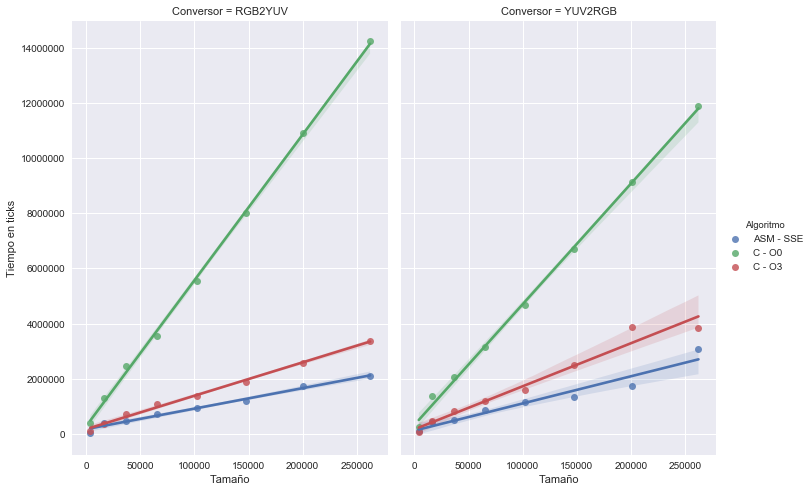
\includegraphics[scale=0.5]{img/conversores_CvsASMvsO3.png}
\end{center}

Lo primero que se puede apreciar en este gráfico es que, más allá de la implementación utilizada, el tiempo de ejecución del filtro aumenta de forma lineal con el tamaño de la imagen, en este caso medido en pixeles. Cabe destacar que en nuestras mediciones, los casos de imágenes pequeñas dieron resultados dispares, pero para el resto de los tamaños esta tendencia se mantiene.

Para continuar, se puede notar una diferencia enorme en la performance del algoritmo escrito en C contra el escrito en ASM. Al compilar con optimizaciones, la brecha de performance baja drásticamente. Sospechamos que esto se debe a un uso más exhaustivo de los registros en lugar de acceder constantemente a memoria. Sin embargo, se puede ver que el algoritmo escrito con instrucciones SIMD sigue siendo más óptimo. Decidimos analizar esto más de cerca:

\begin{center}
	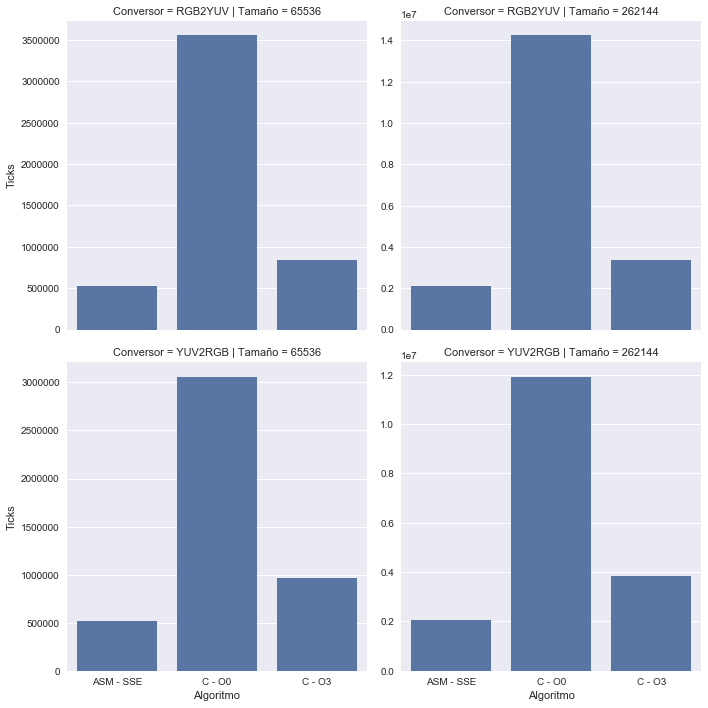
\includegraphics[scale=0.5]{img/conversores_CvsASMvsO3_bars.png}
\end{center}

Este gráfico nos muestra de forma clara que el filtro escrito en ASM se ejecuta en entre 50\% y 70\% del tiempo al compararlo con el filtro en C compilado con el flag \texttt{-O3}. Si bien ambos filtros se ejecutan varias veces más rápido que la versión sin optimizaciones de compilador (\texttt{-O0}), la diferencia porcentual entre ellos es visible y relevante.

Por otro lado, se puede ver que en O0 el conversor YUV a RGB performa mejor que su contraparte RGB a YUV (con una diferencia de más de 10\%). Esto posiblemente se deba a ciertas operaciones que como mencionamos se repiten, y por ende podemos pre-calcular y reutilizar valores intermedios.

\subsection{Experimentación}

A modo de experimentación, decidimos probar 2 hipótesis distintas:

\subsubsection*{Hipótesis 1: cargar 4 pixeles a la vez mejora la performance}

Como se mencionó en la sección de implementación, en nuestra implementación cargamos 4 pixeles de la memoria a los registros XMM, para luego desempaquetarlos y procesarlos de manera individual. Nosotros hicimos esto bajo la hipótesis que reducir los saltos y los accesos a memoria mejoraría el rendimiento de los filtros.

Decidimos comprobar esta teoría implementando los mismos filtros pero cargando y procesando 1 único pixel por iteración:

\begin{center}
	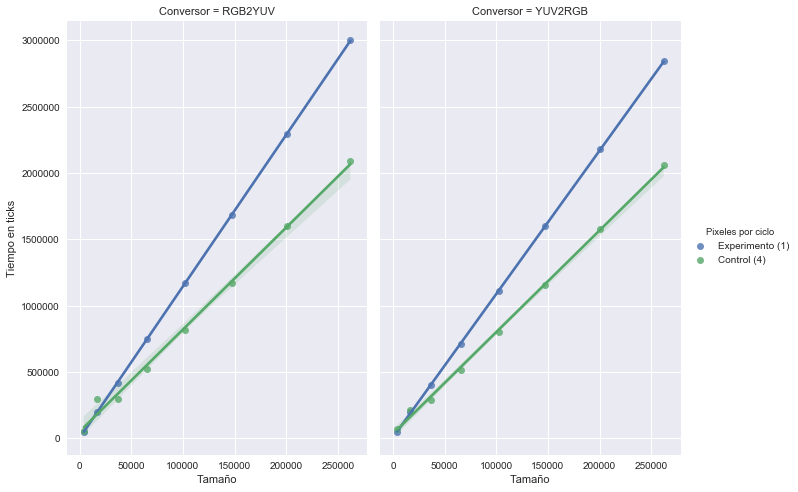
\includegraphics[scale=0.5]{img/conversores_1pixel.png}
\end{center}

Efectivamente, las implementaciones más veloces son aquellas que aprovechan la instrucción \texttt{movdqu} para cargar 4 pixeles con un solo acceso a memoria, y que consecuentemente procesan 4 pixeles sin hacer saltos.

Por otro lado, al acceder de manera lineal a la memoria, el caché debería mitigar una gran candidad de esos accesos, así que es posible que el impacto mayor no provenga necesariamente de los accesos a memoria, sino de los saltos condicionales.

\subsubsection*{Hipótesis 2: los filtros corren en tiempos uniformes para toda imagen de mismo tamaño}

De cara a la experimentación, esperábamos que los algoritmos fuesen agnósticos a la composición de la imagen de entrada, es decir, de los pixeles particulares que la componen. Si bien sabemos que el tamaño de la imagen si afecta de forma lineal el tiempo de ejecución, supusimos que los colores que componen las imágenes no modificarían dicho tiempo.

Para comprobar esta teoría, probamos correr el conversor sobre utilizando un bitmap blanco. Corrimos los mismos conversores, en ambas implementaciones:

\begin{center}
	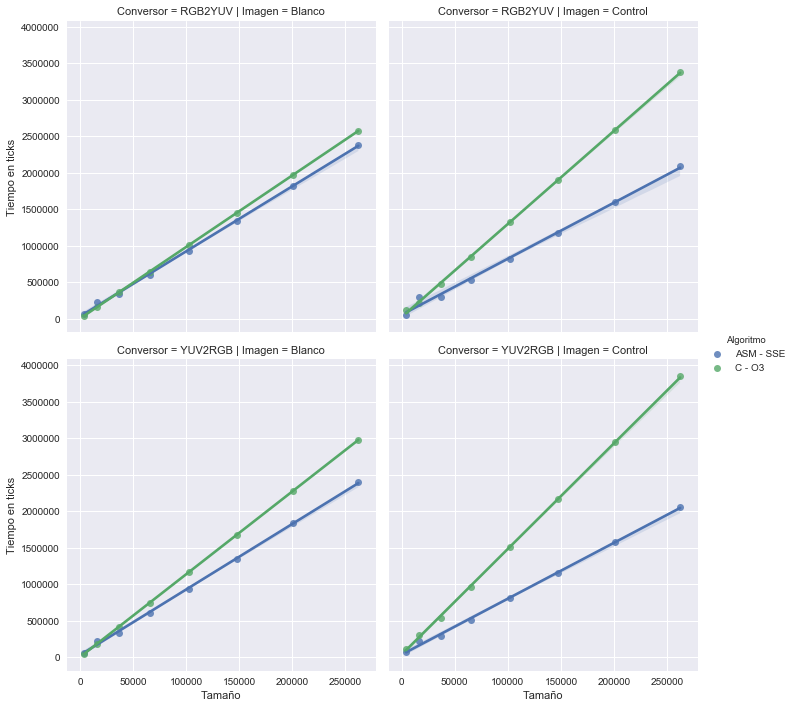
\includegraphics[scale=0.5]{img/conversores_blanco.png}
\end{center}

Para nuestra sorpresa, podemos ver que la saturación de las componentes tiene un efecto visible en el tiempo de ejecución de los filtros. No solo eso, el bitmap afecta de manera positiva a la implementación en C, mientras que impacta de forma negativa a su contraparte SSE.

Este dato nos tomó por sorpresa, y aunque intentamos analizar el por qué de este impacto, no pudimos dilucidar la causa. De un modo u otro, esto muestra que la imagen de entrada pueden afectar notoriamente la performance de los filtros, negando nuestra hipótesis inicial.

% Descripción
% La propiedad lógica descripta sólo dice que la imagen resultante va a tener la misma cantidad de pixeles y el mismo ancho, pero no describe la imagen resultante en cuestión, no le veo mucho sentido.
% La imagen de la transformación está al revés
% Implementación
% La descripción de qué se hace con los punteros a los cuadrantes necesita una re-escritura.
% El código presentado no es claro, qué tienen r10 y r11?
% Análisis preliminar
% No se explica cómo están hechos los experimentos.
% Cómo hicieron el gráfico? Pusieron todos los datos sobre cada ejecución? El gráfico de esta manera puede dar una idea de la varianza, pero no se sabe bien qué tomaron para armar la recta.
% Hipótesis de trabajo
% [DONE] Las consignas, como "Conjunto de ideas de experimentos" indican qué debe ir (no necesariamente tienen que ser títulos).
% [DONE] La comparación entre ASM y C entra dentro de los análisis preliminares.
% Loop unrolling generalmente es aplicado cuando se tiene una cantidad fija de ciclos. Acá lo que hicieron fue hacer un solo unroll del loop, no?
% Experimentación
% La descripción del experimento que les parece interesante debería ir en un apartado "trabajos futuros". Ahí está un poco descolocado.
% El párrafo que comienza con "El roll del cache en imágenes grandes" debería ser re-escrito, tiene varios errores.
% La explicación de lo que se va a medir, debería ser concisa:
% Queremos medir x cosa (el por qué debería estar claro en la hipótesis del trabajo) y cómo lo vamos a hacer.
% Ejemplo (no es para que lo copien literal): Las mediciones se hicieron con tal mecanismo, en tal CPU, tomando la media de los resultados.
% Como nos interesa saber cómo se comportan ambas modificaciones con diferentes tamaños de imágenes, en especial ver cómo se comporta con imágenes más grandes que la caché, utilizamos como entrada imágenes de tamaño x, y, z...
% Para tener un análisis más granular de los tiempos de ejecución de los ciclos, medimos de x manera, con este CPU, z veces y tomamos la media.
% Resultados obtenidos
% El número de la figura al comienzo dice 3 (es 4?)
% El programa pesa más de lo normal? Si se refieren al espacio en memoria que ocupa el código, es muy poco.
% Cuando hacen el análisis del ciclo, cómo lo hicieron? Si el ciclo del unroll es más largo, debería tardar más.
% Sólo incluyan el porcentaje de diferencia, los tics no muestran mucho a simple vista. No queda claro de dónde salió ese 10%, del promedio con las imágenes de distintos tamaños?
% No tiene mucho sentido tener el tiempo de ejecución de C cuando no lo necesitan para su experimentación.
% Conclusiones
% [DONE] Las conclusiones deberían ser generales, al final del informe. El problema de ponerlas en cada filtro es que no pueden sacar conclusiones de todo el trabajo en cuestión.

\section{Combinar}
Este filtro consiste en cambiar la distribución de píxeles de una imagen tal que queden ordenados en cuatro cuadrantes diferentes. Se obtendrá mediante la aplicación de este filtro cuatro imágenes distintas de menor tamaño a la original, pero en donde los píxeles de la original se encuentran aun presentes en la imagen resultante. Es decir: 
\begin{center}
	$\forall$ $pixel,$ $cantidadPixeles(pixel, imagenOriginal) == cantidadPixeles(pixel,imagenResultante)$
	$\wedge$ $imagenOriginal.length == imagenResultante.length$
\end{center}
\begin{flushright}
	$pixel \in imagenOriginal$
\end{flushright}

El resultado visual que provoca la aplicación de este filtro es la sensación de que la imagen se dividió en cuatro pequeñas imágenes cuando verdaderamente ninguna de ella es igual a la otra. 
Se puede ver en el ejemplo de la figura 1 como es la distribución que va teniendo la aplicación de nuestro filtro allí podemos distinguir que los píxeles antes y luego de la aplicación del filtro son los mismos.
\begin{figure}[H]
	\centering
	\begin{subfigure}[b]{0.27\textwidth}
		\centering
		\begin{tikzpicture}
		    [%%%%%%%%%%%%%%%%%%%%%%%%%%%%%%
		        box/.style={rectangle,draw=black,thick, minimum size=1cm},
		    ]%%%%%%%%%%%%%%%%%%%%%%%%%%%%%%
		\draw[step=1cm,color=gray] (-2,-2) grid (2,2);
		\node[box, fill=red] at (-1.5,+1.50) {P1};
		\node[box, fill=red] at (-0.50,+1.50) {P2};
		\node[box, fill=orange] at (+0.50,+1.50) {P3};
		\node[box, fill=orange] at (+1.5,+1.50) {P4};
		\node[box, fill=red] at (-1.5,+0.50) {P5};
		\node[box, fill=red] at (-0.50,+0.50) {P6};
		\node[box, fill=orange] at (+0.50,+0.50) {P7};
		\node[box, fill=orange] at (+1.50,+0.50) {P8};
		\node[box, fill=yellow] at (-1.50,-0.50) {P9};
		\node[box, fill=yellow] at (-0.50,-0.50) {P10};
		\node[box] at (+0.50,-0.50) {P11};
		\node[box] at (+1.50,-0.50) {P12};
		\node[box, fill=yellow] at (-1.50,-1.50) {P13};
		\node[box, fill=yellow] at (-0.50,-1.50) {P14};
		\node[box] at (+0.50,-1.50) {P15};
		\node[box] at (+1.50,-1.50) {P16};
		\end{tikzpicture}
	\end{subfigure}
	{\LARGE$\xrightarrow{FourCombine}$}
	\begin{subfigure}[b]{0.27\textwidth}
		\centering
		\begin{tikzpicture}
		    [%%%%%%%%%%%%%%%%%%%%%%%%%%%%%%
		        box/.style={rectangle,draw=black,thick, minimum size=1cm},
		    ]%%%%%%%%%%%%%%%%%%%%%%%%%%%%%%
		\draw[step=1cm,color=gray] (-2,-2) grid (2,2);
		\node[box, fill=red] at (-1.5,+1.50) {P1};
		\node[box, fill=orange] at (-0.50,+1.50) {P3};
		\node[box, fill=red] at (+0.50,+1.50) {P2};
		\node[box, fill=orange] at (+1.5,+1.50) {P4};
		\node[box, fill=yellow] at (-1.5,+0.50) {P9};
		\node[box] at (-0.50,+0.50) {P11};
		\node[box, fill=yellow] at (+0.50,+0.50) {P10};
		\node[box] at (+1.50,+0.50) {P12};

		\node[box, fill=red] at (-1.50,-0.50) {P5};
		\node[box, fill=orange] at (-0.50,-0.50) {P7};
		\node[box, fill=red] at (+0.50,-0.50) {P6};
		\node[box, fill=orange] at (+1.50,-0.50) {P8};

		\node[box, fill=yellow] at (-1.50,-1.50) {P13};
		\node[box] at (-0.50,-1.50) {P15};
		\node[box, fill=yellow] at (+0.50,-1.50) {P14};
		\node[box] at (+1.50,-1.50) {P16};
		\end{tikzpicture}
	\end{subfigure}
	\caption{Distribución de píxeles tras aplicar el filtro de combinar}
\end{figure}

También podemos ver en la figura 2 cual es el impacto de nuestro filtro en una imagen real, podremos notar aquí lo parecidas que son imágenes resultantes en cada uno de los cuadrantes, a nuestro ojo es casi imperceptible la diferencia.

\begin{figure}[H]
	\centering
	$\vcenter{\hbox{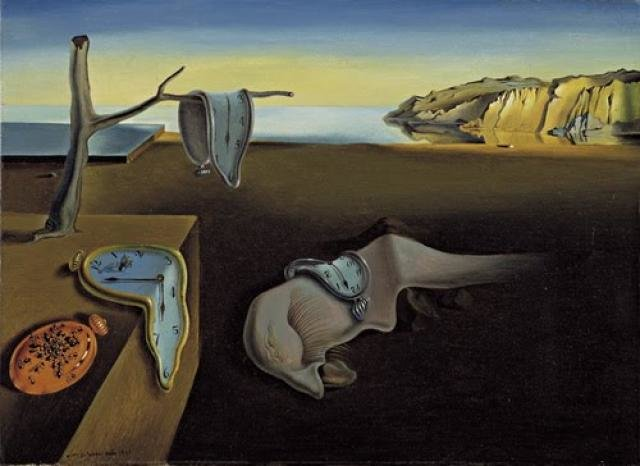
\includegraphics[scale=0.38]{img/fourCombine_before.jpg}}}$
	$\vcenter{\hbox{\LARGE$\xrightarrow{\text{T}}$}}$
	$\vcenter{\hbox{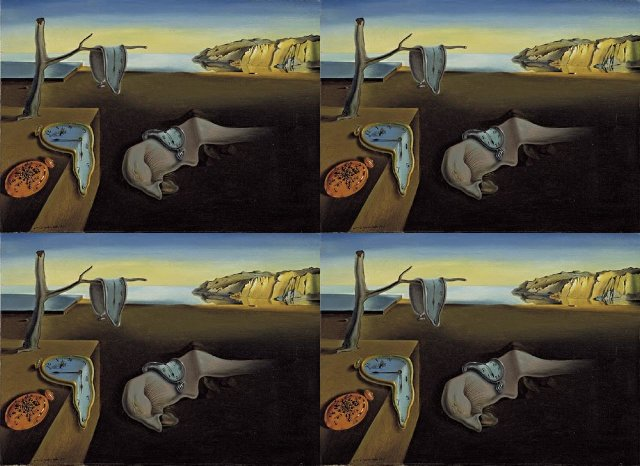
\includegraphics[scale=0.38]{img/fourCombine_after.jpg}}}$

	\caption{Imagen real antes y luego de la aplicación del filtro}
\end{figure}

\subsection{Implementación}
\paragraph{Solución en código C}
La solución que fue planteada en c consiste en recorrer la matriz asociada a la imagen de entrada una sola vez píxel por píxel. Cada uno de estos píxeles posee una coordenada y por medio de esta se calcula la coordenada en la matriz asociada a la imagen de salida. 


\paragraph{Solución en ASM}
En cuanto a la implementación en código assembler se tuvo que pensar una solución totalmente diferente ya que al tener que hacerlo con registros de 128 bits nuestra solución de agarrar los píxeles uno por uno y calcular su lugar correspondiente no seria posible. Se tomaron las siguientes decisiones de modelado Decisiones de modelado:
\begin{itemize}
\item Decidir con cuanta información a la vez íbamos a trabajar , se llego a la conclusión que lo mejor seria trabajar con 8 píxeles a la vez. Esta decisión se tomo puesto que eligiendo los 8 píxeles del lugar correcto podíamos llegar a armar 8 píxeles que iban a ser puestos en la imagen de salida. Esto nos debería dar un ahorro en la cantidad de veces que vamos a pegarle a memoria.
\item Decidir entre la posibilidad de agarrar 16 píxeles que este en la misma fila o que estén la misma columna. Nos pareció lo mas fácil de implementar y lo mas efectivo a la hora de usar la cache era que tomáramos 8 píxeles contiguos. Se vera mas adelante en un experimento la diferencia entre ambos
\item Ya que íbamos a tomar de a 8 píxeles contiguos pero el enunciado del trabajo practico solo aseguraba que la imagen a lo ancho iba a ser múltiplo de 4 , teníamos que hacer algo con respecto a los casos donde la imagen no era múltiplo de 8. En este caso tratamos de emular un poco la practica que realiza muchas veces el compilador de intel donde este separa el código en casos especiales para poder ahorrarse de preguntar en el medio del código . Por ende en nuestro código ASM solo preguntamos una vez si el ancho es múltiplo de 4 o de 8 y dependiendo de eso el código se disfurca en dos
\end{itemize}

Ahora hablemos un poco mas de la iteración dentro del un ciclo de nuestro código ASM , podemos separar lo que hace dentro de una columna de lo que hace al cambiar de fila. Dentro de una columna nuestro objetivo es agarrar 8 píxeles llámense $Pi$ con $1\leq i\leq 8$ y trabajarlos de forma tal que queden listos para ser pegados en la memoria de la imagen destino. El siguiente gráfico nos mostrara como ocurre la transformación de los 8 píxeles desde que son extraídos desde la imagen fuente hasta que están listos para ser puestos en la imagen destino:

\begin{center}
	\begin{tikzpicture}
		\matrix [matrix of nodes,row sep=,row sep=0mm,
		column 1/.style={nodes={rectangle,draw,minimum width=3em}},
		column 2/.style={nodes={rectangle,draw,minimum width=3em}},
		column 3/.style={nodes={rectangle,draw,minimum width=3em}},
		column 4/.style={nodes={rectangle,draw,minimum width=3em}},
		] (P)
		{
		P8 & P7 & P6 & P5\\
		};
	\end{tikzpicture}
	\begin{tikzpicture}
		\matrix [matrix of nodes,row sep=,row sep=0mm,
		column 1/.style={nodes={rectangle,draw,minimum width=3em}},
		column 2/.style={nodes={rectangle,draw,minimum width=3em}},
		column 3/.style={nodes={rectangle,draw,minimum width=3em}},
		column 4/.style={nodes={rectangle,draw,minimum width=3em}},
		] (P)
		{
		P4 & P3 & P2 & P1\\
		};
	\end{tikzpicture}
\end{center}

Separo en pares e impares

\begin{center}
	\begin{tikzpicture}
	\matrix [matrix of nodes,row sep=,row sep=0mm,
	column 1/.style={nodes={rectangle,draw,minimum width=3em}},
	column 2/.style={nodes={rectangle,draw,minimum width=3em}},
	column 3/.style={nodes={rectangle,draw,minimum width=3em}},
	column 4/.style={nodes={rectangle,draw,minimum width=3em}},
	] (P)
	{
	0 & P7 & 0 & P5\\
	};
	\end{tikzpicture}
	\begin{tikzpicture}
	\matrix [matrix of nodes,row sep=,row sep=0mm,
	column 1/.style={nodes={rectangle,draw,minimum width=3em}},
	column 2/.style={nodes={rectangle,draw,minimum width=3em}},
	column 3/.style={nodes={rectangle,draw,minimum width=3em}},
	column 4/.style={nodes={rectangle,draw,minimum width=3em}},
	] (P)
	{
	0 & P3 & 0 & P1\\
	};
	\end{tikzpicture}

	\begin{tikzpicture}
	\matrix [matrix of nodes,row sep=,row sep=0mm,
	column 1/.style={nodes={rectangle,draw,minimum width=3em}},
	column 2/.style={nodes={rectangle,draw,minimum width=3em}},
	column 3/.style={nodes={rectangle,draw,minimum width=3em}},
	column 4/.style={nodes={rectangle,draw,minimum width=3em}},
	] (P)
	{
	P8 & 0 & P6 & 0\\
	};
	\end{tikzpicture}
	\begin{tikzpicture}
	\matrix [matrix of nodes,row sep=,row sep=0mm,
	column 1/.style={nodes={rectangle,draw,minimum width=3em}},
	column 2/.style={nodes={rectangle,draw,minimum width=3em}},
	column 3/.style={nodes={rectangle,draw,minimum width=3em}},
	column 4/.style={nodes={rectangle,draw,minimum width=3em}},
	] (P)
	{
	P4 & 0 & P2 & 0\\
	};
	\end{tikzpicture}
\end{center}

Shifteo pre juntar

\begin{center}
	\begin{tikzpicture}
	\matrix [matrix of nodes,row sep=,row sep=0mm,
	column 1/.style={nodes={rectangle,draw,minimum width=3em}},
	column 2/.style={nodes={rectangle,draw,minimum width=3em}},
	column 3/.style={nodes={rectangle,draw,minimum width=3em}},
	column 4/.style={nodes={rectangle,draw,minimum width=3em}},
	] (P)
	{
	P7 & 0 & P5 & 0\\
	};
	\end{tikzpicture}
	\begin{tikzpicture}
	\matrix [matrix of nodes,row sep=,row sep=0mm,
	column 1/.style={nodes={rectangle,draw,minimum width=3em}},
	column 2/.style={nodes={rectangle,draw,minimum width=3em}},
	column 3/.style={nodes={rectangle,draw,minimum width=3em}},
	column 4/.style={nodes={rectangle,draw,minimum width=3em}},
	] (P)
	{
	0 & P4 & 0 & P2\\
	};
	\end{tikzpicture}
\end{center}

Los uno cruzados con un or

\begin{center}
	\begin{tikzpicture}
	\matrix [matrix of nodes,row sep=,row sep=0mm,
	column 1/.style={nodes={rectangle,draw,minimum width=3em}},
	column 2/.style={nodes={rectangle,draw,minimum width=3em}},
	column 3/.style={nodes={rectangle,draw,minimum width=3em}},
	column 4/.style={nodes={rectangle,draw,minimum width=3em}},
	] (P)
	{
	P7 & P3 & P5 & P1\\
	};
	\end{tikzpicture}
	\begin{tikzpicture}
	\matrix [matrix of nodes,row sep=,row sep=0mm,
	column 1/.style={nodes={rectangle,draw,minimum width=3em}},
	column 2/.style={nodes={rectangle,draw,minimum width=3em}},
	column 3/.style={nodes={rectangle,draw,minimum width=3em}},
	column 4/.style={nodes={rectangle,draw,minimum width=3em}},
	] (P)
	{
	P8 & P4 & P6 & P2\\
	};
	\end{tikzpicture}
\end{center}

Hago shuffle 

\begin{center}
	\begin{tikzpicture}
	\matrix [matrix of nodes,row sep=,row sep=0mm,
	column 1/.style={nodes={rectangle,draw,minimum width=3em}},
	column 2/.style={nodes={rectangle,draw,minimum width=3em}},
	column 3/.style={nodes={rectangle,draw,minimum width=3em}},
	column 4/.style={nodes={rectangle,draw,minimum width=3em}},
	] (P)
	{
	P7 & P5 & P3 & P1\\
	};
	\end{tikzpicture}
	\begin{tikzpicture}
	\matrix [matrix of nodes,row sep=,row sep=0mm,
	column 1/.style={nodes={rectangle,draw,minimum width=3em}},
	column 2/.style={nodes={rectangle,draw,minimum width=3em}},
	column 3/.style={nodes={rectangle,draw,minimum width=3em}},
	column 4/.style={nodes={rectangle,draw,minimum width=3em}},
	] (P)
	{
	P8 & P6 & P4 & P2\\
	};
	\end{tikzpicture}
\end{center}


Una vez que tenemos los 8 píxeles ordenados según los quiero procedo a guardarlos en la posiciones de memoria a las que apuntan el registro $R8$ y $R9$ sin preocuparme en este caso del cuadrante donde estos dos están apuntando.

En cuando a que pasa cuando la iteración sobre la columna se termina y se pasa a una nueva columna lo vamos a explicar a continuación:
Primero movemos $R8$ y $R9$ hacia su próxima fila recordando que la próxima fila sea cual sea el cuadrante donde se encuentro se realiza sumándole una fila a cada uno.

El tema viene ahora en que hay que ir switcheando los cuadrantes donde voy insertando los píxeles resultantes cada uno fila. Siendo esta parte del código la que se encarga de swtichear $R8$ y $R9$ entre los distintos cuadrantes se utiliza para ello una variable puente para no sobrescribir ni pisar ningún valor. 

Snippet del código :

\begin{lstlisting}
	mov rax, r8
	mov r8, r10
	mov r10, rax
	mov rax, r9
	mov r9, r11
	mov r11, rax
\end{lstlisting}

Lo único que cambia de esta explicación con respecto a cuando el ancho no es multiplico de 8 es en este punto donde tenemos que cambiar de fila, ya que nos quedaron 4 píxeles sin procesar y como seria demasiado trabajoso holdearlos para poder trabajarlos en otra iteración posterior, lo mejor que nos ocurrió fue trabajarlos manualmente e insertarlos en el lugar donde les corresponde. Luego de esto se sigue con el paso recién explicado.


\subsection{Análisis preliminar}

\begin{figure}[H]
	\centering
	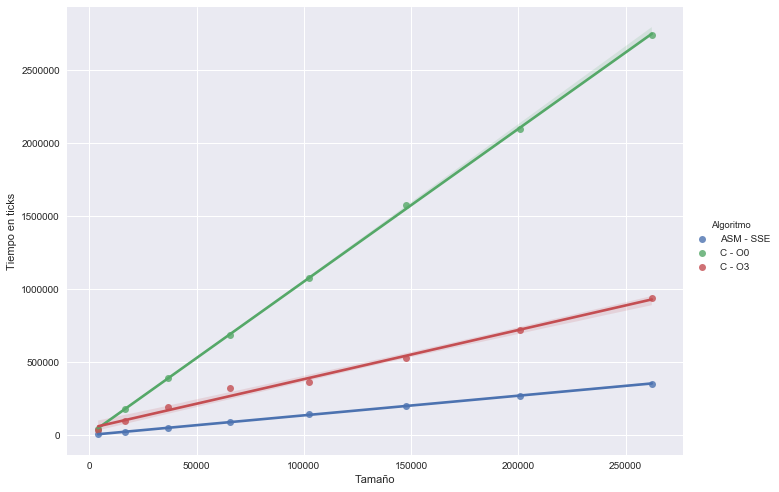
\includegraphics[scale=0.5]{img/fourCombine_CvsASMvsO3.png}
	\caption{Comparación llana de las implementaciones en C contra la implementación en ASM}
\end{figure}

Luego de sacar manualmente un poco del ruido podemos ver una clara diferencia entre la implementación de C y la de ASM. Dato curioso que podemos agregar entre la diferencia de O0 y O3 es que al momento de compilar con gcc ( gracias a la herramienta \url{https://godbolt.org/} ) se puede apreciar como una linea de código se vuelve ASM dependiendo el flag. 

Después de analizarlo los resultados tanto en O0 como en O3 podemos ver que esta linea de código :

\begin{lstlisting}
		mDst[offsetH + (h >> 1)][offsetW + (w >> 1)] = mSrc[h][w];
\end{lstlisting}

Cuando se encuentra el flag de O0 activado $h >> 1$ se calcula todas las veces, en cambio cuando el flag de O3 esta activo esto no sucede y se calcula antes de ciclar. Existen otras mejoras pero el nivel del código no nos permitió encontrarlas. Nos pareció interesante en este gráfico dejar todos tiempos que fuimos midiendo para ver que tal se comporta el ordenador cuando medimos tiempos aunque hay un poco de outliners la gran mayoría de los tiempos rondan en lo mismo.

\subsection{Hipótesis de trabajo}

Una de las primeras ideas a la hora de experimentar con nuestra implementación de ASM es poder correrla en contra de la de implementación que se realizo en C , teniendo en cuenta que en el caso de este filtro juega mas el echo de guardar en memoria los datos que de procesarlos.

También tratamos de llevar a cabo en este conjunto de experimentación la idea de Loop unrolling , con alguna pequeña modificación. Si vamos a lo que se entiende como Loop unrolling y lo aplicamos al algoritmo de ASM lo que lograríamos seria leer de a 16 píxeles a lo largo a la vez en de a 8 píxeles logrando así una reducción en los saltos del loop de columna. Pero esta implementación nos llevaría a tener que abrir mas los casos en los cuales anteriormente tratábamos ahora tendríamos imágenes que deberían ser congruentes a 0 modulo 16 para poder ir por el camino del unrolling pero caso contrario es decir ser congruente 4, 8 , 12 deberían tratarse en otra parte del programa y así solo logrando un incremento en la performance para 0.25 de los casos. Para poder solventar este pequeño numero de casos donde el unrolling podría ser efectivo se decidió procesar 16 píxeles a la vez pero distribuidos en dos filas , de esta manera solo habría que tener en cuenta que las filas sean múltiplos de 2 es decir pares para poder aplicar esta mejora al algoritmo.

Otra idea que había surgido para probar en un experimento fue la de usar registros mas grandes (AVX) para poder lograr así una reducción a la hora de mezclar los elementos, se había pensado que teniendo muchos mas píxeles juntos iba a resultar mas fácil poder ordenarlos para su posterior puesta en en memoria. El problema con este experimento fue que encontramos que las instrucciones AVX (que funcionan en 256 bits) lo único que hacen es replicar comportamientos en la parte baja y la alta del registro es decir los trata como dos registros de 128 bits que solo logran comportamientos de este tipo de registro. Desistimos de hacer este experimento por no encontrar las instrucciones necesarias para poder realizar un código mas performante que el propuesto como solución.

Buscamos mediante distintos sistemas de medidas mostrar que desenrollar el loop aumenta la performance de nuestro algoritmo ya que el sistema de predicción debería predecir menos saltos.

\subsection{Diseño experimental}

Queremos ver bien de cerca que es lo que pasa con nuestras dos implementaciones porque si tomamos las medidas en una escala muy chica vamos a perder información sobre que lo que esta pasando. 

También nos gustaría saber cual es el tiempo que se demoran ambos algoritmos en desarrollar un ciclo. Sabemos que la diferencia esta en que ambos resuelven diferente cantidad de  píxeles a la vez, por ende el tiempo que demoren en resolver un ciclo va a estar dividido por la cantidad de elementos que trabaja a la vez. Vamos a poner también en la misma linea el tiempo de un ciclo del algoritmo de c que solo procesa un píxel a la vez.

Un experimento interesante que debería estar incluido en el tp sería poder medir que porcentaje de un ciclo del algoritmo presentado como respuesta se utiliza cargando datos, que porcentaje en procesarlos y que porcentaje en cargarlos nuevamente a memoria, tenemos la impresión que la gran mayoría del tiempo se la pasa cargando y poniendo cosas en memoria por ende si quisiéramos mejorar aun mas nuestro algoritmo podríamos solamente trabajar sobre el porcentaje de procesamiento de los datos. Estaríamos en presencia de un cuello de botella representado por la memoria.

El roll del cache en imágenes grandes aquí vamos a probar cual es la diferencia entre la implementación presentada como respuesta al trabajo practico y la implementación del unrolling. Aunque anteriormente vimos que en ejemplos chicos la implementación del unrolling era mejor, en el caso de imágenes obscenamente grandes (mayores a la capacidad del cache) esto no ocurre en imágenes grandes.

En el único momento que vamos a utilizar datos por fuera de la cátedra va a ser al momento de querer ver el funcionamiento de la cache en nuestro algoritmo, en este caso utilizamos una imagen que excede la cache de nuestra CPU , la imagen pesa 200mb y por obvios motivos no va a ser adjuntada junto al tp.

\subsection{Resultados y Análisis}

\begin{figure}[H]
	\centering
	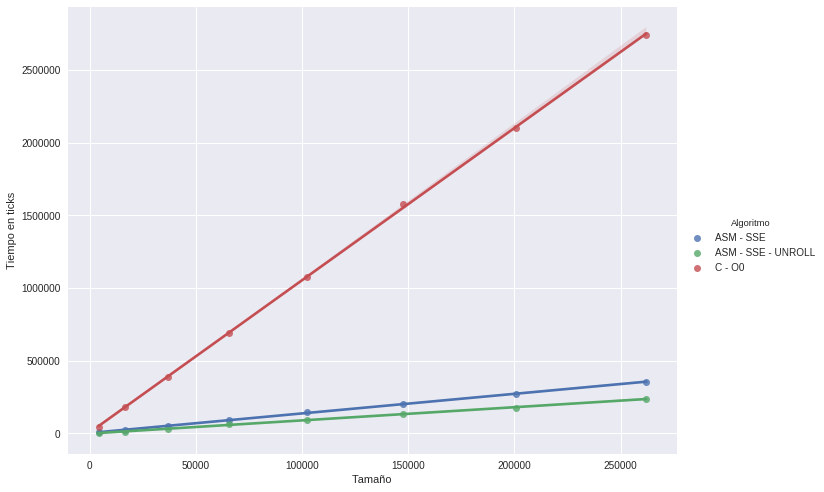
\includegraphics[scale=0.5]{img/fourCombine_UnrollvsNormal.png}
	\caption{Versión Unroll del algoritmo puesta en comparación del entregado como respuesta del tp}
	\label{sec:unroolvsnormal}
\end{figure}

\begin{figure}[H]
	\centering
	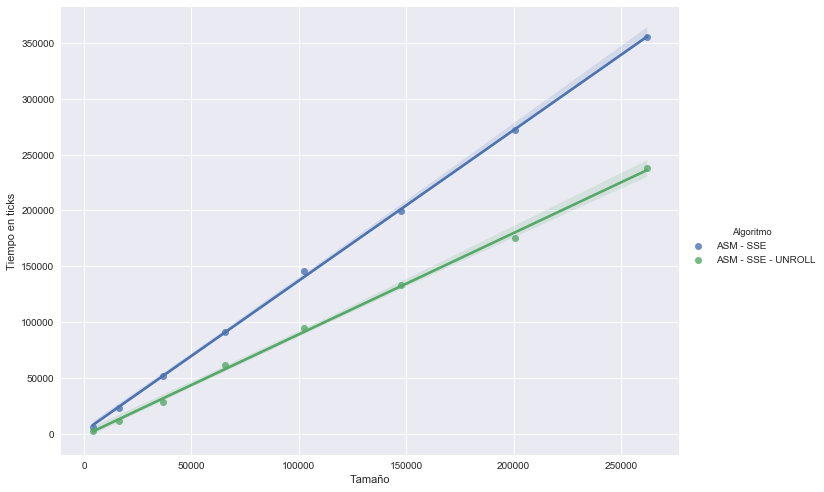
\includegraphics[scale=0.5]{img/fourCombine_UnrollvsNormal_asmOnly.png}
	\caption{Comparación exclusiva de las implementaciones en ASM}
	\label{sec:unroolvsnormal_asmOnly}
\end{figure}

\begin{figure}[H]
	\centering
	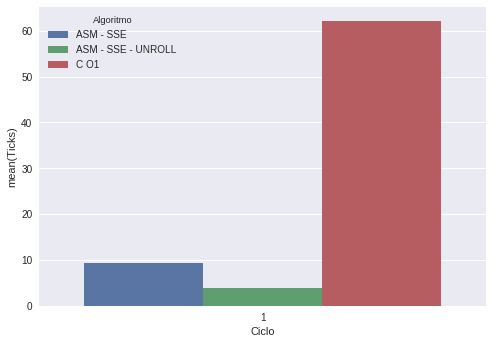
\includegraphics[scale=0.5]{img/fourCombine_ticks_en_ciclo.png}
	\caption{Ticks en un ciclo comparación de las 3 implementaciones}
	\label{sec:ticksciclo}
\end{figure}

Podemos distinguir de la figura 3 que hay una mejora a medida que la imagen se va haciendo cada vez mas grande en el algoritmo de desarrollo del ciclo, esto nos estaría indicando a simple vista que el método funciona, podríamos tener alguna desventaja ya que nuestro programa estaría pesando mas de lo normal, pero esto no sería algo que tenga importancia en un programa como el desarrollado. También se puede hablar de la comparación en imágenes chicas viendo la figura 4. En este caso se trabajo con los resultados mas chicos del set de resultados para poder ver que tan distintos o iguales eran los algoritmos y se puede notar que en imágenes chicas no hay casi diferencia de performance, esto tiene sentido pensando que en imágenes chicas no existe una cantidad de saltos que pueda llegar a influir en la predicción de saltos del procesador.

Por ultimo una manera interesante de ver la diferencia de la performance que se nos ocurrió fue la de medir un ciclo de cada algoritmo y ver que tan performante era cada uno luego de hacer la modificación a esto como se indica en la sección de "como y que van a medir" se puede observar otra manera como la implementación de UNROLL lograr obtener un tiempo que es al menos dos veces mejor que el método puesto en nuestro TP. Este resultado parece contradecir los anteriores dos ya que en estos no se observa que los resultados del UNROLL sean dos veces mejores. No fue testeado pero mi hipótesis recae a que el trabajo que se debe hacer cada vez que se cambia de fila es mayor cuando estamos haciendo el UNROLL , tal vez por la misma ineficiencia de la implementación. Pero este resultado nos muestra el potencial que tiene el UNROLL al poder tener un mejor tiempo de procesamiento por píxel.

Por ultimo voy a hablar de mi test sobre la cache sobre el cual solo quedan los resultados y no hay gráfico asociado . Temo que la  hipótesis que teníamos no se pudo probar ya que los mejores tiempo tanto para el código ASM original como para el ASM - UNROLL son los siguientes :  $243442734$ ticks y $220905687$ ticks respectivamente , hay una mejora de al menos $10\%$ en promedio , cuando se esperaba que al poder leer por filas en nuestro ASM original se podría conseguir una hit rate mas grande. 
\subsection{Conclusiones}
En conclusión el unroll aplicado al algoritmo original logro aumentar la performance mas denotada en imágenes mas grandes. El poder procesar mas píxeles hace que el ciclo sea mas corto y por lo tanto es ahí donde gana tiempo. El algoritmo se podría mejorar para evitar perder tanto tiempo cuando se cambia de fila.

\section{Zoom}

El filtro LinearZoom consiste en interpolar linealmente los pixeles de la imagen, duplicando su ancho y su alto, es decir aumentando su tamaño efectivo en 4.

La interpolación lineal de los pixeles consiste en calcular los promedios de cada componente entre los pixeles adyacentes al nuevo pixel interpolado. La misma se puede representar con la siguente matriz:

\begin{table}[H]
  \centering
  \begin{tabular}{ | c | c | }
    \hline
    A & B \\ \hline
    C & D \\
    \hline
  \end{tabular}
  {\LARGE$\xrightarrow{LinearZoom}$}
  \begin{tabular}{ | c | c | c | c |}
    \hline
    A & (A+B)/2 & B & $\cdots$ \\ \hline
    (A+C)/2 & (A+B+C+D) & (B+D)/2 & $\cdots$ \\ \hline
    C & (C+D)/2 & D & $\cdots$ \\ \hline
    $\vdots$ & $\vdots$ & $\vdots$ & $\ddots$ \\
    \hline
  \end{tabular}
\end{table}

En el caso de la última fila y la última columna, como no existe información para interpolar, los elementos deben ser duplicados.

El filtro en sí no presenta un efecto visual muy notorio, pero el tamaño de la imagen crece.

\subsection{Implementación}

En la implementación en C, un detalle con el que nos cruzamos y que nos generó errores fue que la imagen se encuentra alamcenada con las filas inferiores en primer lugar. Esto es, si representamos la imagen como un arreglo bidimensonal de pixeles \texttt{RGBA** img}, esto significa que \texttt{img[0][0]} contiene el primer pixel de la fila inferior de la imagen.

Por como dividimos el problema (se detalla más adelante), esto generó confusión al implementar los casos especiales del filtro. No obstante, esto nos sirvió para estructurar mejor la implementación en ASM, que por la naturaleza de ese lenguaje resulta más compleja.

En la implementación con SIMD, podemos aprovechar las operaciones vectoriales para operar no solo sobre las múltiples componentes a la ves, sino también sobre más de un pixel (como son sumas de hasta 4 bytes, solo requerimos tamaño word por componente).

Nuestra implementación en particular procesa los pixeles en el siguiente orden (donde w es el ancho y h la altura en pixeles):

\begin{center}
  \begin{tabular}{ | c | c | c | c | c | c |}
    \hline
    w & w-1 & $\cdots$ & 3 & 2 & 1 \\ \hline
    2*w & 2*w-1 & $\cdots$ & w+3 & w+2 & w+1 \\ \hline
    $\vdots$ & $\vdots$ & $\ddots$ & $\vdots$ & $\vdots$ & $\vdots$ \\ \hline
    w*h & w*h-1 & $\cdots$ & w*(h-1)+3 & w*(h-1)+2 & w*(h-1)+1 \\
    \hline
  \end{tabular}
\end{center}

Este orden fue escogido en su momento por resultar más sencillo de implementar, pero es posible que el orden de operación resulte en menos comparaciones y saltos condicionales.

El filtro puede dividirse en 4 secciones, dependiendo de la posición en la imagen del pixel a procesar:

\begin{enumerate}
  \item Caso general: la gran mayoría de los pixeles entran en esta categoría. En estos casos, se deben cargar 4 pixeles de la memoria para procesar y crear 3 pixeles interpolados (como se muestra en la tabla anterior).

  Los 4 pixeles a procesar (que llamaremos A, B, C y D como figuran en la tabla anterior) son cargados en 2 accesos a memoria, ya que pertenecen a 2 filas distintas de la imagen de origen:

  \begin{center}
    \xmm{0} \xmmDoubleWordSmall{0}{0}{B}{A}

    \xmm{1} \xmmDoubleWordSmall{0}{0}{D}{C}
  \end{center}

  Los mismos son desempaquetados para ocupar los registros enteros en esa misma disposición.

  Por un lado, calculamos los dos pixeles que resultan de interpolar 2 pixeles de origen:

  \begin{center}

    \xmm{3} \xmmQuadWord{B}{A}

    \texttt{MOVLHPS} \xmm{3}, \xmm{3} \hfill

    \xmm{3} \xmmQuadWord{A}{A}

    \xmm{4} \xmmDoubleWordSmall{0}{0}{B}{A}

    \xmm{5} \xmmDoubleWordSmall{0}{0}{D}{C}

    \texttt{PSRLDQ} \xmm{4}, 4 \hfill

    \texttt{PSLLDQ} \xmm{5}, 4 \hfill

    \xmm{4} \xmmDoubleWordSmall{0}{0}{0}{B}

    \xmm{5} \xmmDoubleWordSmall{0}{D}{C}{0}

    \texttt{PADDB} \xmm{4}, \xmm{5} \hfill

    \xmm{4} \xmmDoubleWordSmall{0}{D}{C}{B}

    \texttt{PUNPCKLBW} \xmm{4}, CEROS \hfill

    \xmm{4} \xmmQuadWord{C}{B}

    \texttt{PADDW} \xmm{3}, \xmm{4} \hfill

    \xmm{3} \xmmQuadWord{A+C}{A+B}

    \texttt{PSRLW} \xmm{4}, 1 \hfill

    \xmm{3} \xmmQuadWord{(A+C)/2}{(A+B)/2}
  \end{center}

  Por el otro, calculamos el pixel que proviene de interpolar 4 pixeles a la vez:

  \begin{center}
    \xmm{0} \xmmQuadWord{B}{A}

    \xmm{1} \xmmQuadWord{D}{C}

    \texttt{PADDW} \xmm{1}, \xmm{0} \hfill

    \xmm{1} \xmmQuadWord{B+D}{A+C}

    \xmm{0} $\leftarrow$ \xmm{1}

    \texttt{PSRLDQ} \xmm{1}, 8 \hfill

    \xmm{1} \xmmQuadWord{0}{B+D}

    \texttt{PADDW} \xmm{1}, \xmm{0} \hfill

    \xmm{1} \xmmQuadWord{B+D}{A+B+C+D}

    \texttt{PSRLW} \xmm{1}, 2 \hfill

    \xmm{1} \xmmQuadWord{(B+D)/4}{(A+B+C+D)/4}
  \end{center}

  Por último, empaquetamos y ordenamos los pixeles de la siguiente forma:

  \begin{center}
    \xmm{2} \xmmDoubleWord{(A+B+C+D)/4}{(A+C)/2}{(A+B)/2}{A}
  \end{center}

  Al igual que en la carga, los resultados empaquetados son guardados a memoria de a 2, ya que pertenecen a distintas filas de la imagen de destino. Los dos pixeles de la parte baja del registro corresponden a la fila superior de la imagen, mientras que los dos pixeles alta del registro corresponden a la fila interior de la imagen.

  \item Última columna: en estos casos los pixeles B y D del diagrama no existen, por lo que solo se calcula 1 pixel interpolado entre A y C, y tanto A como el nuevo pixel generado son duplicados a la derecha.

  El proceso es similar al caso general, obteniendo como resultado:

  \begin{center}
    \xmm{2} \xmmDoubleWordSmall{0}{0}{(A+C)/2}{(A+C)/2}
  \end{center}

  Sin embargo, se omiten las operaciones que utilizan B y D cuando se puede, y se asumen ceros en sus lugares. Además, el pixel original se copia duplicado por separado.

  \item Última fila: similar al caso de última columna, los pixeles C y D no existen. A es interpolado con B, y tanto A como el nuevo pixel generado son duplicados hacia abajo.

  % \begin{center}

  %   \xmm{0} \xmmQuadWord{B}{A}

  %   \xmm{1} $\leftarrow$ \xmm{0}

  %   \texttt{MOVLHPS} \xmm{1}, \xmm{1} \hfill

  %   \xmm{1} \xmmQuadWord{A}{A}

  %   \texttt{PADDW} \xmm{0}, \xmm{1} \hfill

  %   \xmm{0} \xmmQuadWord{A+B}{A+A}

  %   \texttt{PSRLW} \xmm{0}, 1 \hfill

  %   \xmm{0} \xmmQuadWord{(A+B)/2}{A}

  % \end{center}

  El proceso es similar al caso general, obteniendo como resultado:

  \begin{center}
    \xmm{2} \xmmDoubleWordSmall{0}{0}{(A+B)/2}{A}
  \end{center}

  Sin embargo, se omiten las operaciones que utilizan B y D cuando se puede, y se asumen ceros en sus lugares. Ambos pixeles son duplicados en la última fila de la imagen destino.

  \item Último pixel: este caso refiere a un pixel ubicado en última fila y columna. Aqui no hay pixel para interpolar, por lo que se hace un cuadruplicado de A.

  \begin{center}

    \xmm{15} \xmmDoubleWordSmall{0}{0}{0}{A}

    \xmm{14} $\leftarrow$ \xmm{15}

    \texttt{PSLLDQ} \xmm{14}, 4 \hfill

    \xmm{14} \xmmDoubleWordSmall{0}{0}{A}{0}

    \texttt{PADDB} \xmm{15}, \xmm{14} \hfill

    \xmm{15} \xmmDoubleWordSmall{0}{0}{A}{A}

  \end{center}

\end{enumerate}

\subsection{Análisis preliminar}

Dado que la interpolación lineal es un procesamiento muy conocido de imágenes, nos esperabamos que fuese uno de los filtros más beneficiados por la vectorización de los cálculos.

\begin{center}
  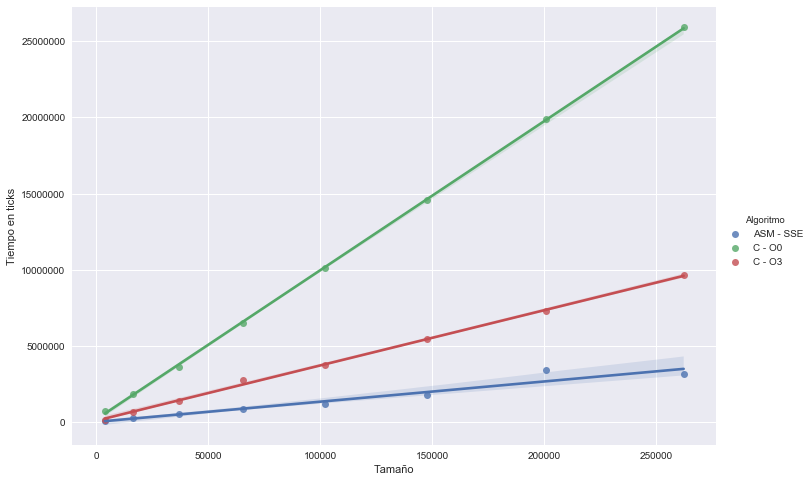
\includegraphics[scale=0.5]{img/linearZoom_CvsASMvsO3.png}
\end{center}

Por un lado, podemos observar que, como el resto de los filtros, el tiempo de ejecución de los filtros crece de forma lineal respecto a la cantidad de pixeles. Esto es esperable, ya que por cada pixel del caso general se deben leer y escribir 4 pixeles. Eso no es así para los otros pixeles, pero en nuestros tests de control estos representan la menor parte. Es posible que en imágenes pequeñas con distintas proporciones (por ejemplo, 200x50 en lugar de 100x100) esta proporción no se respete, pero el impacto de los casos borde debería ser menor a medida que crece la imagen.

\begin{center}
  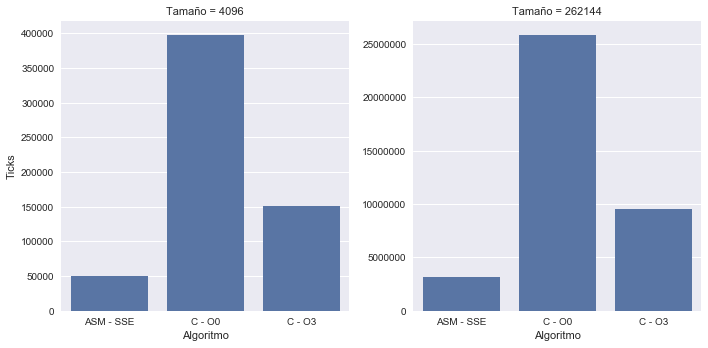
\includegraphics[scale=0.5]{img/linearZoom_CvsASMvsO3_bars.png}
\end{center}

Por otro lado, podemos ver que efectivamente, incluso con las optimizaciones de GCC, la vectorización de la interpolación aumenta el rendimiento de manera dramática, ejecutando el filtro siempre en menos del 40\% del tiempo.

\subsection{Experimentación}

Como se mencionó en la sección de implementación, nosotros utilizamos \texttt{mov}s, shifts y \texttt{add}s para acomodar los pixeles y realizar los promedios entre los pixeles. Sin embargo, existen instrucciones específicamente pensadas para estas tareas: los shuffles y los blends.

Con esto en mente, decidimos modificar nuestro filtro para que utilice dichas instrucciones:

\begin{center}
  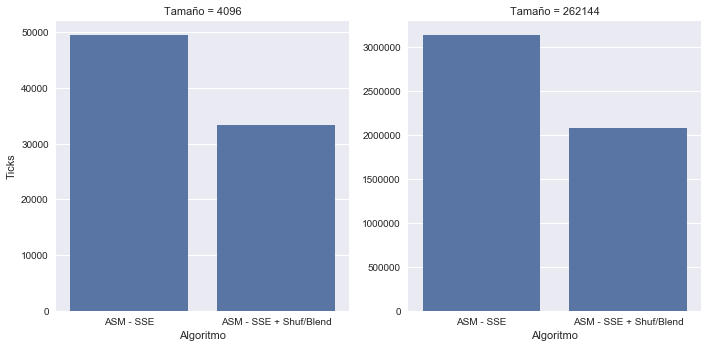
\includegraphics[scale=0.5]{img/linearZoom_shuf_bars.png}
\end{center}

Nuestras pruebas confirmaron esta hipótesis: en promedio pudimos reducir el tiempo de ejecución en 30\%. Nuestra idea es que usar instrucciones como \texttt{pshufd} y \texttt{pblendw} es más eficientes porque combinan la copia y el acomodado de los pixeles a los bits específicos de los registros que necesitamos. Al mismo tiempo evitamos utilizar la parte lógica del CPU, ya que no utilizamos add sino blend para mezclar los registros, y suponemos que requiere menos tiempo de espera que una suma de números empaquetados.

\section{Maximo cercano}

%[DONE]Descripción:
%	Fijensé si no queda mejor utilizar enumerates para describir los pasos a realizar para aplicar el filtro.[DONE]
%[DONE]Implementación:
%	Necesitaría una re-escritura. Es difícil de seguir a veces, no es muy clara.[DONE]
%	Al principio describís lo que parecería ser el filtro en C. La división entre la explicación de cada implementación no queda muy clara.[DONE]
%	Dicen que utilizan 4 píxeles en un registro, y 4 en el otro. No describen si son contiguos o si es la fila inferior.[DONE]
%Análisis preliminar
%	No tiene mucho sentido tener dos gráficos, uno con O3 y otro sin O3. [DONE]
%	Sería interesante tener como resultado cuán mejor en tiempo una implementación contra la otra. [DONE]
%Experimentación
%	Lo que quieren ver es cuán diferente va a ser temporalmente cada una de las implementaciones, y eso no está claro en los gráficos.
%		No hablan sobre alguna característica observable en el gráfico en relación al tamaño de la entrada, sólo comentan cuántas veces más rápido es.
%		No está claro con ver en los gráficos que es 2.5, 1.4, o 1.2 veces más rápido, deberían cambiarlos por otros donde la comparación sea evidente. Lo que comentan debe estar respaldado y ser fácil de corroborar a simple vista.
%	Falta experimentación.

Este es un filtro tal que cada pixel de la imagen original se edita de la siguiente manera:

\begin{enumerate}
	\item Obtenemos los píxeles de alrededor, que se encuentren a una distancia menor a 3 píxeles.
	\item Se calcula el máximo valor para cada componente entre estos píxeles obtenidos.
	\item Se genera un nuevo píxel con estas 3 valores encontrados.
	\item El píxel final se calcula mediante una combinación lineal entre el píxel original y el píxel que contiene las componentes máximas.
\end{enumerate}

El conjunto de píxeles en donde se busca el máximo valor de cada componente, se lo conoce como kernel y en este caso es de 7x7 píxeles.\\
La combinación lineal entre los píxeles se hace de la siguiente manera:

\begin{center}
	$src * (1 - val) + max * (val)$
\end{center}

Donde $src$ es el píxel original, $max$ es el píxel generado, y $val$ es un número flotante entre 0 y 1, este mismo es un parámetro del filtro.

\begin{table}[h]
\centering
\begin{tabular}{l|c|c|c|c|c|c|c|l}
 & \multicolumn{1}{l|}{}       & \multicolumn{1}{l|}{}      & \multicolumn{1}{l|}{}       & \multicolumn{1}{l|}{}       & \multicolumn{1}{l|}{}       & \multicolumn{1}{l|}{}       & \multicolumn{1}{l|}{}      &  \\ \hline
 & \cellcolor[HTML]{FAFE8E}$P_{00}$ & \cellcolor[HTML]{FAFE8E}$P_{01}$  & \cellcolor[HTML]{FAFE8E}$P_{02}$  & \cellcolor[HTML]{FAFE8E}$P_{03}$  & \cellcolor[HTML]{FAFE8E}$P_{04}$  & \cellcolor[HTML]{FAFE8E}$P_{05}$ & \cellcolor[HTML]{FAFE8E}$P_{06}$ &  \\ \hline
 & \cellcolor[HTML]{FAFE8E}$P_{10}$ & \cellcolor[HTML]{FAFE8E}$P_{11}$  & \cellcolor[HTML]{FAFE8E}$P_{12}$  & \cellcolor[HTML]{FAFE8E}$P_{13}$  & \cellcolor[HTML]{FAFE8E}$P_{14}$  & \cellcolor[HTML]{FAFE8E}$P_{15}$ & \cellcolor[HTML]{FAFE8E}$P_{16}$ &  \\ \hline
 & \cellcolor[HTML]{FAFE8E}$P_{20}$ & \cellcolor[HTML]{FAFE8E}$P_{21}$  & \cellcolor[HTML]{FAFE8E}$P_{22}$  & \cellcolor[HTML]{FAFE8E}$P_{23}$  & \cellcolor[HTML]{FAFE8E}$P_{24}$  & \cellcolor[HTML]{FAFE8E}$P_{25}$ & \cellcolor[HTML]{FAFE8E}$P_{26}$ &  \\ \hline
 & \cellcolor[HTML]{FAFE8E}$P_{30}$ & \cellcolor[HTML]{FAFE8E}$P_{31}$  & \cellcolor[HTML]{FAFE8E}$P_{32}$  & \cellcolor[HTML]{FE8E8E}$P_{33}$  & \cellcolor[HTML]{FAFE8E}$P_{34}$  & \cellcolor[HTML]{FAFE8E}$P_{35}$ & \cellcolor[HTML]{FAFE8E}$P_{36}$ &  \\ \hline
 & \cellcolor[HTML]{FAFE8E}$P_{40}$ & \cellcolor[HTML]{FAFE8E}$P_{41}$  & \cellcolor[HTML]{FAFE8E}$P_{42}$  & \cellcolor[HTML]{FAFE8E}$P_{43}$  & \cellcolor[HTML]{FAFE8E}$P_{44}$  & \cellcolor[HTML]{FAFE8E}$P_{45}$ & \cellcolor[HTML]{FAFE8E}$P_{46}$ &  \\ \hline
 & \cellcolor[HTML]{FAFE8E}$P_{50}$ & \cellcolor[HTML]{FAFE8E}$P_{51}$  & \cellcolor[HTML]{FAFE8E}$P_{52}$  & \cellcolor[HTML]{FAFE8E}$P_{53}$  & \cellcolor[HTML]{FAFE8E}$P_{54}$  & \cellcolor[HTML]{FAFE8E}$P_{55}$ & \cellcolor[HTML]{FAFE8E}$P_{56}$ &  \\ \hline
 & \cellcolor[HTML]{FAFE8E}$P_{60}$ & \cellcolor[HTML]{FAFE8E}$P_{61}$  & \cellcolor[HTML]{FAFE8E}$P_{62}$  & \cellcolor[HTML]{FAFE8E}$P_{63}$  & \cellcolor[HTML]{FAFE8E}$P_{64}$  & \cellcolor[HTML]{FAFE8E}$P_{65}$ & \cellcolor[HTML]{FAFE8E}$P_{66}$ &  \\ \hline
 & \multicolumn{1}{l|}{}      & \multicolumn{1}{l|}{}      & \multicolumn{1}{l|}{}       & \multicolumn{1}{l|}{}       & \multicolumn{1}{l|}{}       & \multicolumn{1}{l|}{}       & \multicolumn{1}{l|}{}      &
\end{tabular}
\caption{Kernel, en rojo el pixel que estamos editando y en amarillo los píxeles que forman parte del kernel}
\end{table}


\subsection{Implementación}

Para la implementación de este filtro, recorremos la imagen original, iterando sobre sus filas y sus columnas, como hay píxeles que no tenemos un kernel de 7x7 alrededor, estos los pintamos de blanco, pero si podemos, iteramos sobre el kernel y nos vamos fijando cuáles son las componentes máximas y cuando recorrimos todo el kernel, para cada componente hacemos esta cuenta: \\ Componente Destino $\leftarrow$ Componente Original * (1 - VAL) + Componente Máxima * VAL. (Donde VAL es el parámetro que nos pasan en la función).
 
La implementación en C se trató de hacerla lo más simple posible. Iteramos las filas y las columnas, y en cada paso preguntamos si el píxel se encuentra en el margen de 3 píxeles, si es así, lo pintamos de blanco, y si no, nos generamos un píxel con cada componente inicializada en el mínimo valor(0) y recorremos el kernel y usamos este píxel que acabamos de generar para usarlo de máximo actual, entonces vamos modificando cada componente cuando encontramos un valor mayor al encontrado, una vez iterado el kernel realizamos la combinación lineal sobre cada componente y guardamos el píxel en la imagen destino.
 
En cambio, en la implementación del filtro en lenguaje ensamblador, esta se ve complejizada ya que podemos aprovechar de las ventajas que nos brinda el modelo SIMD. En particular, los registros XMM son de 16 bytes, que los podemos utilizar para procesar 4 píxeles en paralelo. Para esta implementación, vamos a aprovechar estos registros para buscar el máximo sobre el kernel y hacer la combinación lineal sobre cada componente en paralelo.
 
En este caso también vamos a iterar sobre las filas y las columnas, primero recorremos las filas y vamos a diferenciar 2 casos, el caso en que toda la fila se encuentra en el margen que se pinta de blanco y el que no.
 
Si es una fila blanca, vamos a intentar guardar la mayor cantidad de píxeles contiguos posible, como ya vimos que en los registros XMM nos caben 4, nos generamos un registro tal que los 4 píxeles sean blancos y guardarlos en memoria a la vez, al ser imágenes con ancho múltiplo de 4, podemos aplicar esto sobre toda la fila, entonces iteramos sobre las columnas pero vamos aumentando en 4 el índice de la columna. Con esto logramos en las primeras filas y las últimas una reducción al iterar las columnas.
 
Ahora sí es una fila que no va a pertenecer en su completitud al margen, vamos a tener que calcular el máximo de cada color en el kernel y después hacer la combinación lineal. En la iteración del kernel, en diferencia a C, podemos guardarnos 4 píxeles tal que puedan ser los máximos, vamos a hacer uso de la instrucción PMAXUB, que compara byte a byte entre los registros y guarda el máximo en el registro destino. Gracias a esta instrucción podemos ir comparando estos 4 posibles máximos contra 4 píxeles contiguos del kernel (notar que la comparación es byte a byte, así que va a comparar las componentes), e ir manteniendo los máximos. Como en el kernel tenemos nada más 7 píxeles contiguos, vamos a aplicar este método 2 veces por fila, repitiendo un píxel de la fila en cada aplicación total esto no va a afectar el resultado.

\begin{figure}[H]
	\centering
	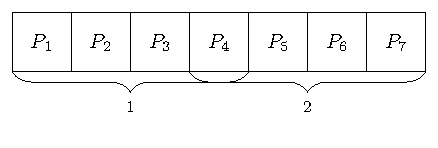
\includegraphics{img/max/filaKernel.pdf}
	\caption{Píxeles contiguos de una fila del kernel, las llaves indican que píxeles se toman en las 2 aplicaciones por fila}
\end{figure}

\begin{center}

	\xmm{1} \xmmDoubleWordSmall{$P_1$}{$P_2$}{$P_3$}{$P_4$}

	\xmm{2} \xmmDoubleWordSmall{$P_5$}{$P_6$}{$P_7$}{$P_8$}

	\texttt{PMAXUB} \xmm{1}, \xmm{2} \hfill

	\xmm{1} \xmmDoubleWordSmall{\tiny$MAX(P_1,P_5)$}{\tiny$MAX(P_2,P_6)$}{\tiny$MAX(P_3,P_7)$}{\tiny$MAX(P_4,P_8)$}

	$MAX(PM,P)$ = \xmmDoubleWordSmall{\tiny$MAX(PM^r,P^r)$}{\tiny$MAX(PM^g,P^g)$}{\tiny$MAX(PM^b,P^b)$}{\tiny$MAX(PM^a,P^a)$}
\end{center}

Una vez realizado esto sobre cada fila, vamos a tener en el registro los cuatro posibles píxeles máximos, ahora debemos compararlos entre sí para conseguir el píxel que contenga el máximo de cada componente. Para esto podemos seguir usando PMAXUB, duplicamos el registro y shifteamos 8 bytes a la derecha uno de ellos, para que nos quede desplazado 2 píxeles y podamos comparar el primer par de píxeles del registro contra el segundo par. Todavía nos queda por comparar 2 píxeles así que repetimos este procedimiento pero esta vez desplazamos un solo píxel, una vez realizado esto nos va a quedar en la parte menos significativa del registro el píxel que estábamos buscando.

\begin{center}
	\xmm{1} \xmmDoubleWordSmall{$M_1$}{$M_2$}{$M_3$}{$M_4$}

	\xmm{2} $\leftarrow$ \xmm{1}

	\texttt{PSRLDQ} \xmm{2}, \texttt{8} \hfill

	\xmm{2} \xmmDoubleWordSmall{0}{0}{$M_1$}{$M_2$}

	\texttt{PMAXUB} \xmm{1}, \xmm{2} \hfill

	\xmm{1} \xmmDoubleWordSmall{$M_1$}{$M_2$}{\tiny$MAX(M_1,M_3)$}{\tiny$MAX(M_2,M_4)$}

	\xmm{2} $\leftarrow$ \xmm{1}

	\texttt{PSRLDQ} \xmm{2}, \texttt{4} \hfill

	\xmm{2} \xmmDoubleWordSmall{0}{$M_1$}{$M_2$}{\tiny$MAX(M_1,M_3)$}

	\texttt{PMAXUB} \xmm{1}, \xmm{2} \hfill

	\xmm{1}
	\vspace{0.1cm}
	\begin{tabular}{|C{1cm}|C{1cm}|C{1cm}|C{3.8cm}|}\hline
		X & X & X & $MAX(M_1,M_2,M_3,M_4)$ \\ \hline
	\end{tabular}
	\vspace{0.1cm}
\end{center}

Ya conseguido el máximo, ahora tenemos que realizar la combinación lineal con el píxel original, el nuevo píxel que generamos y el parámetro. Lo que queremos es hacer la cuenta para cada componente paralelo, para eso, podemos usar instrucciones SIMD para multiplicar las componentes de los píxeles en paralelo por el parámetro, que es un float, entonces convertimos a float cada componente quedándonos todas las componentes en un registro XMM, y para multiplicarlas por el parámetro tenemos que hacer un registro XMM que lo contenga 4 veces y aplicamos MULPS, quedando de resultado la multiplicación por cada componente contra el parámetro cada una en floats. Luego hacemos lo mismo con el píxel original, y sumamos estos dos resultados. Ahora nos queda guardar este resultado en la imagen destino, pero antes, debemos convertir los floats a integers. Ya guardado en memoria, podes seguir repitiendo el paso para los otros píxeles.

\subsection{Análisis preliminar}

\begin{center}
	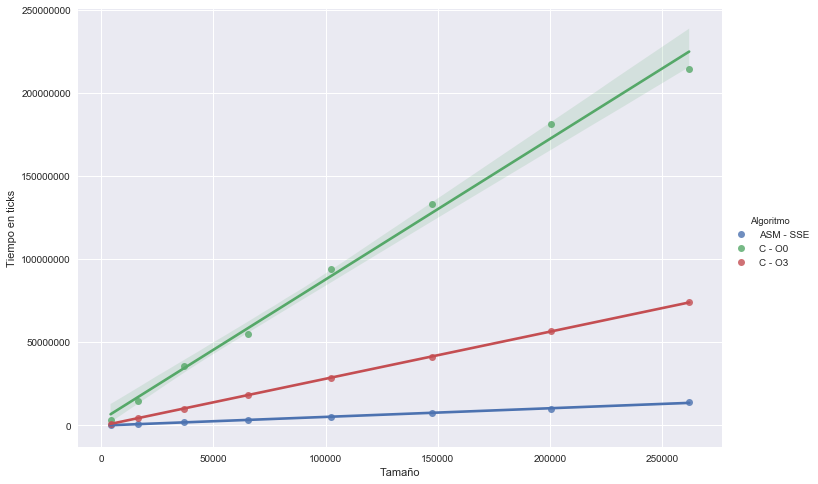
\includegraphics[scale=0.5]{img/maxCloser_CvsASMvsO3.png}
\end{center}

Podemos ver claramente como el filtro implementado en ASM corre más rápido que en C, de hecho, al incrementar el tamaño de la imagen la diferencia es aún más notable. Si bien hay una amplia mejora al compilar con optimizaciones \texttt{-O3}, no llega a mejorar la versión de ASM.

\begin{center}
	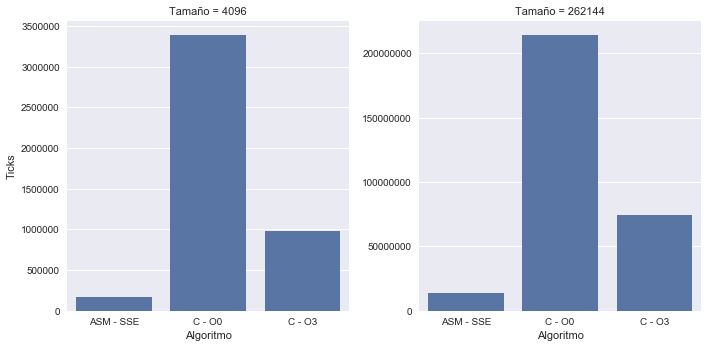
\includegraphics[scale=0.5]{img/maxCloser_CvsASMvsO3_bars.png}
\end{center}

Analizando de cerca, podemos ver que la diferencia entre las distintas implementaciones es la mayor entre todos los filtros estudiados: la implementación en ASM corren en menos de 25\% del tiempo en promedio para una misma imagen.

Esto es un comportamiento esperable ya que en C estamos yendo a buscar el pixel a memoria por cada pixel del kernel, en cambio en ASM con las instrucciones SIMD cada 7 pixeles lo pedimos 2 veces. Además, en ASM aprovechamos y hacemos las cuentas para el pixel destino en paralelo.

\subsection{Experimantación}
Como reveló el análisis preliminar, la cantidad de pixeles origen a procesar por pixel destino tuvo un gran impacto en la performance de nuesto filtro. Decidimos ver cómo impacta en ambas implementaciones si agrandamos el tamaño de kernel. Para esto corrimos los mismos tests que antes, pero ahora con un kernel de 11x11 en vez que de 7x7.

Nuestra hipótesis fue que esta medida afectaría con más contundencia a la implementación de C, si bien en ASM va a tardar más, en relación al kernel mas chico, no le va afectar tanto. Esto es debido a que en C trae cada pixel del kernel uno por vez, y como estamos incrementando el tamaño del kernel en casi 2.5 veces, esperamos una performance peor en este orden. Pero en ASM aprovechando la paralelización de datos, levantamos 11 píxeles con 3 llamadas a memoria nada más.

% TODO: medir esto de nuevo, asegurarse de usar O3, conservar datos en jupyter

\begin{center} 
	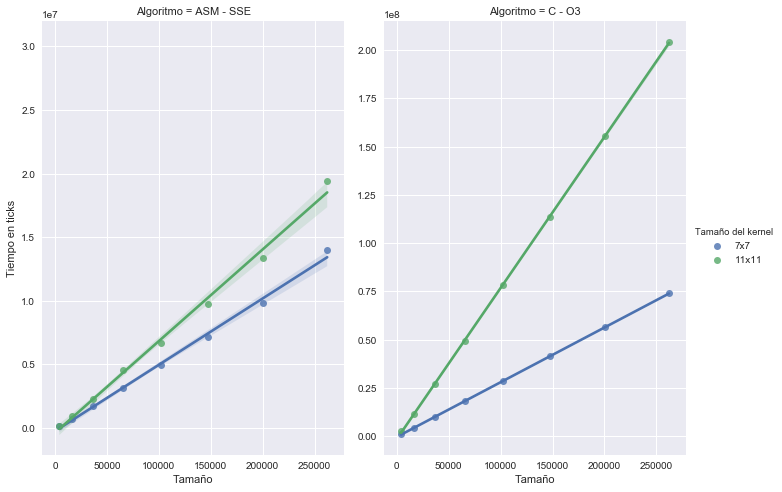
\includegraphics[scale=0.5]{img/maxCloser_KERNEL.png}
	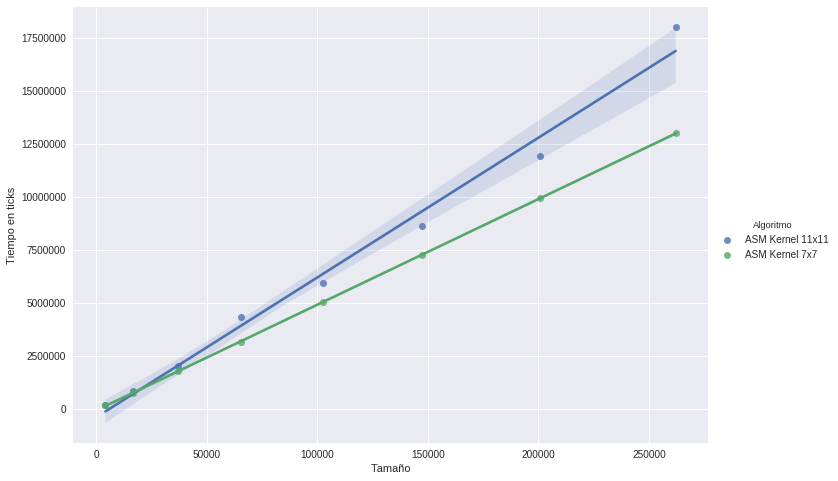
\includegraphics[scale=0.5]{img/maxCloser_KERNEL_ASM.png}
	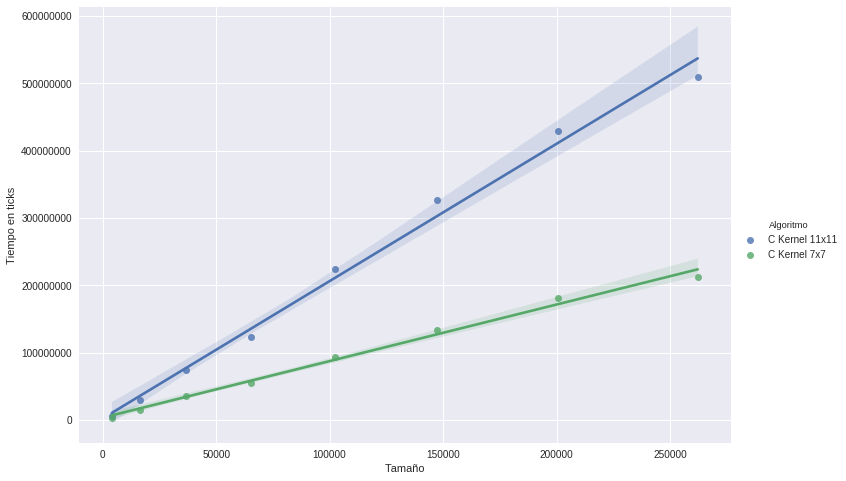
\includegraphics[scale=0.5]{img/maxCloser_KERNEL_C.png}
\end{center}

Si observamos los gráficos, podemos ver como en C con el kernel de 11x11 tarda casi 2.5 veces más, como la relación de diferencia de pixeles en los kernels, y para ASM hay nada mas una diferencia de 1.2 y 1.4 para instancias más grandes. Como habíamos predicho en la hipótesis, este cambio en el tamaño del kernel afectó bastante más a la implementación de C que a la de ASM.

\subsubsection*{Análisis de las variables de entrada}

Queremos realizar un análisis sobre el tiempo en que tarda en terminar el filtro en base a los parámetros que recibe, distintos tipos de imagen, tamaños y el valor que afecta la combinación lineal. Nuestra hipótesis es que las pruebas que hacemos no van a tener un impacto significativo sobre el rendimiento del filtro, ya que no hay optimizaciones que hagan variar el tiempo final según los parámetros(si la cantidad de píxeles como vimos en el análisis preliminar).

Primero hagamos un análisis sobre distintas imágenes y cómo reacciona el algoritmo frente a ellas, en este caso vamos a comparar las imágenes de lena y colores (las de los tests de la cátedra), una de los siguientes colores azul, rojo, verde, gris, blanco y negro y por último una imagen generada aleatoriamente(en python), donde cada píxel es de un color elegido aleatoriamente distribuido uniformemente. Para la experimentación se dejó fijo en todas las imágenes el tamaño(512x512), el valor de la combinación final en 0.5, y se corrió la experimentación unas 100 veces y para cada color nos quedamos con el que menor tiempo resultó.

\begin{center} 
	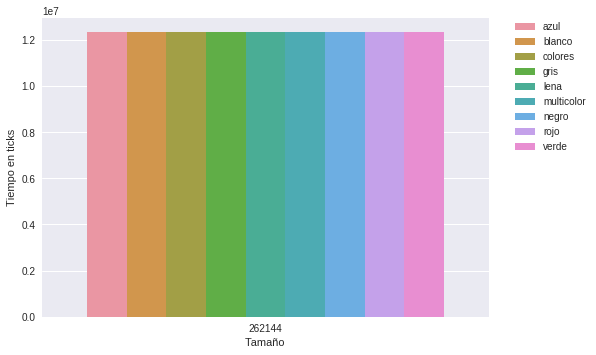
\includegraphics[scale=0.5]{img/maxCloser_PARAM_IMG.png}
\end{center}

A simple vista se ve que varía muy poco, y posiblemente esto sea producto de la inexactitud de la experimentación. Este resultado se debe a que los cálculos se hacen de cualquier manera, siempre buscamos en el kernel el mayor de las componentes, una cosa que se nos ocurrió es que la imagen aleatoria podría haber llegado a tardar un poco más debido a que cambia más el valor del máximo en la búsqueda del kernel, no como en los colores fijos que no cambia, pero suponemos que esto no tiene impacto y que el procesador no pierde más tiempo cuando por ejemplo en la instrucción pmaxub tiene que cambiar los valores en los registros.

El siguiente experimento fue sobre el parámetro de entrada de punto flotante que se aplica sobre la combinación lineal, notemos que acá si podríamos haber optimizado cuando el valor viene en 0 ya que nos podemos ahorrar la búsqueda del máximo, pero es una optimización simple que no es a lo que apuntamos en este trabajo. Corrimos este experimento como en el anterior pero para las imágenes de lena y colores y variamos el valor entre los siguientes 0 0.313 0.5 0.713 1.

\begin{center} 
	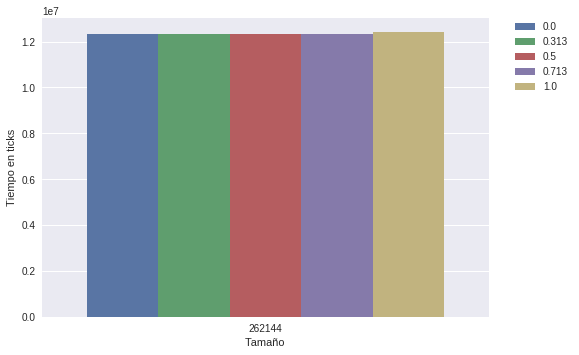
\includegraphics[scale=0.5]{img/maxCloser_PARAM_VAL.png}
\end{center}

De nuevo podemos observar la poca varianza entre los distintos valores, el que menos ticks dió fue el de 0.5 con 12335487 ticks y el que mayor fue el de 1 con 12416301 ticks, la diferencia entre estos dos representa el $0,65\%$ de este último. Con estos resultados podemos afirmar que no hay diferencia significativa.

Por último probamos cómo afectan las diferentes proporciones de tamaño, básicamente queremos ver como afecta si la imagen es más ancha que alta, en este caso probamos para las imágenes de lena y colores,  con el valor fijo en 0.5 y probamos para tamaños de 512x128 y 128x512 ya que tienen la misma cantidad de píxeles.

\begin{center} 
	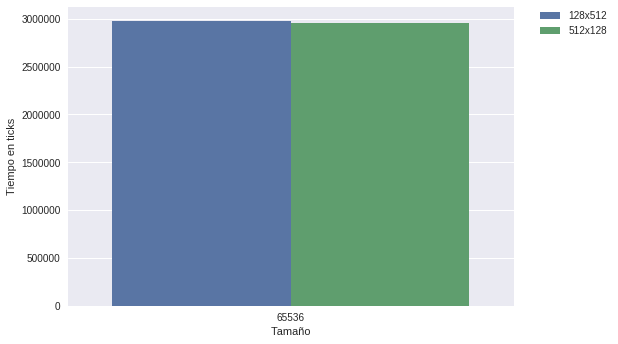
\includegraphics[scale=0.5]{img/maxCloser_PARAM_SIZE.png}
\end{center}

Esta vez vemos una leve mejora en el que es más ancho, 2975394 vs 2956806, el ancho corre en el $99.3\%$, la verdad que es un muy poca la diferencia, esto podría provenir de dibujar las primeras 3 filas y las ultimas son mas fácil de pintar porque no se calcula nada(las filas blancas) y si son más anchas, vamos a poner mas pixeles dentro de estas(la cantidad de píxeles blancos es la misma pero en el otro están concentrados en las primeras y últimas columnas) 

\subsubsection*{Unrolling}

En este experimento, nuevamente aplicamos la técnica de unrolling de ciclos, sobre el kernel, cuando estamos ciclando las filas, ya que nuestro kernel tiene una cantidad constantes de filas, y gracias a esto podemos aplicar esta técnica. Pero no como en el experimento que ya aplicamos esta técnica, tenemos la hipótesis de que la mejora será muy leve o nula, esto lo suponemos ya que el grueso del cómputo del filtro está en las pegadas a memoria, y en comparación a los saltos condicionales del ciclo estos últimos no son relevantes. Corrimos los mismos tests que en el analisis preliminar para la version original y la version con unrolling, ademas agregamos un tamaño de más de 5120x5120.

\begin{center} 
	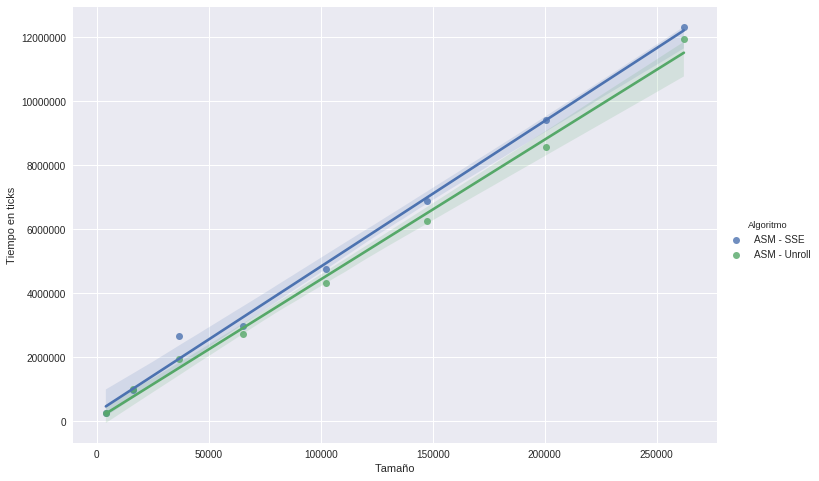
\includegraphics[scale=0.5]{img/maxCloser_Unroll_compare.png}
	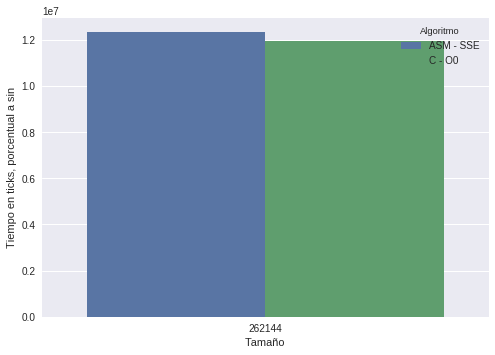
\includegraphics[scale=0.5]{img/maxCloser_Unroll_small.png} %512x512
	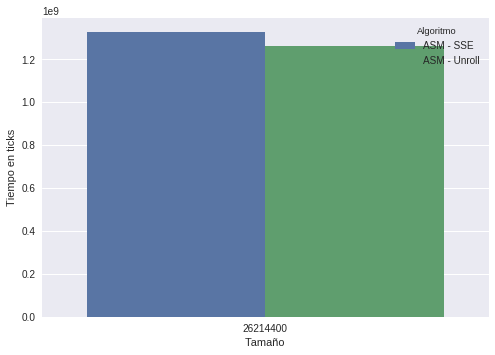
\includegraphics[scale=0.5]{img/maxCloser_Unroll_big.png} %5120x5120
\end{center}

Hay una mejora, pero en comparación a lo que tarda el algoritmo es muy poca, para la imagen de 512x512 resulto en una mejora del $4\%$ y y para la imagen de 5120x5120 hay una mejora del $5\%$, que no es mucho pero si estamos en una imagen muy grande o tenemos que optimizar mucho podria llegar a valer la pena.

\end{document}